\section{Experimental Analysis}

I have implemented several algorithms and each algorithm are dependent on different parameters, which makes it difficult to make a one-factor-at-a-time analysis. Instead I try to be as structured as possible to test what algorithm, objective function, network structure and network type (BNN or TNN), that works best. 
I divide the experimental analysis into several sections. At first I only test on the well-known MNIST dataset, which is a large database of handwritten digits. The dataset contains 60,000 training images and 10,000 testing images. Each image is a $28 \times 28$ grayscale image of a handwritten digit. At the end of the experimental analysis I take the knowledge gained about what parameters work best for MNIST and try to see how it works on different datasets. The first section will be concentrated about single batch training, which could be relevant in few-shot learning. Here the goal is to test what objective function works best, how the amount of data influences the accuracy and what the effect of the network size is. This section will only use the ILS algorithm outlined in Algorithm \ref{ils}. Some of the network architectures tested will be identical to those of \cite{icarte2019} and \cite{thorbjarnason2023}, such that a comparison can be made. At the end a small hyper-parameter study will be conducted to see how sensitive the algorithm is to the choice of $ps$. \\

\noindent The second section is about multiple batch training. Again the goal is to investigate what objective functions work best, but the goal is also to test which of the two algorithms presented for multiple batch training works best. A focus point will also be how the algorithms scale with increasing network size. 
The first two sections will only deal with BNNs. In the third section I will test the TNN, where I speficially aim to investigate whether a regularization parameter help. Another focus point will be how it compare against a BNN, especially if it requires more training time to obtain similar accuracies or not. 
In the fourth section I present the results on the BeMi ensemble introduced by \cite{ambrogio2023}. Here the focus will be how the ensemble works with increasing number of training data, as this is a limitation for their MIP implementation. Lastly, in the fifth section I intend to use the knowledge obtained from the previous four sections to test how the best found algorithms and parameters generalize to other datasets. \\

\noindent The source code for the implementation in Python and experiment scripts can be found at: (GitHub link). For all the experiments, the results reported are an average of 5 runs for each configuration tested. The experiment is run on a Windows 10 computer with a 64-bit operating system with 8 GB RAM. The processor is a Intel(R) Core(TM) i5-6400 CPU with 2.70GHz. 


\subsection{Single Batch Training}

This section will only use the ILS procedure given in Algorithm \ref{ils}. In each perturbation I initially change the value of 25 randomly chosen weights. The first goal is to explore what objective function works best under what circumstances. The first experiment will be to test the influence of more training data, but with a short time limit of only 60 seconds. The second experiment tests how the results develop if the time limit increases. In experiment 3, I test different network architectures and finally in experiment 4, I test how sensitive the results are to the choice of $ps$. For all the experiments in this section, to compare against existing literature, I use a balanced training and test set meaning that the number of instances are equal for each class. The test accuracy is reported on a set of 8,000 instances from the test set, 800 instances for each digit.

\subsubsection{Comparing Objective Functions}

As a starting point I start by testing how the different objective functions compare against each other. The network has a single hidden layer, such that the network structure is $[784, 16, 10]$. I use a BNN with a time limit of 60 seconds. Besides from comparing the objective functions against each other, I also want to see how the results develop as the amount of training data increase and to see this I let the total number of training samples vary from 100 to 2000, or from 10 to 200 examples from each class. In Figure \ref{SBT_COF} I plot the mean of the test accuracy, with the standard deviation as a shaded area around it. Initially as more training samples are added, the accuracy increases a lot, but later on the effect takes of and the accuracy actually decreases at the end. It is possible that the results could be even better with more time, which will be explored in the next experiment. At first the cross entropy objective function works best, but eventually the integer objective function takes over. The objective function based on the Brier score does not seem to be able to compete against the other objective functions. The maximum mean accuracy achieved for this result is with the integer objective function and a batch size of 1800, which gives a mean accuracy of 71.73 \%. \\

\noindent This network architecture is also tested by \cite{thorbjarnason2023}, who only uses a training set of 100 samples, 10 from each digit. Their best performing model gets an average testing accuracy of 51.1 \% with an average runtime of 1852 seconds. With the cross entropy objective function I get a mean testing accuracy of 55.41 \% for the same amount of data, but with a time limit of only 60 seconds. For the integer objective function, the result is a testing accuracy of 49.66 \%. Both of my results may very well be subject to improvement, if the time limit increases. Also, my results are on a pure BNN, while their results are based on a TNN. My results also show that the network architecture, even though it is quite small, can find a model that generalizes better, if the amount of training data increase. 

\begin{figure}[H]
    \centering
    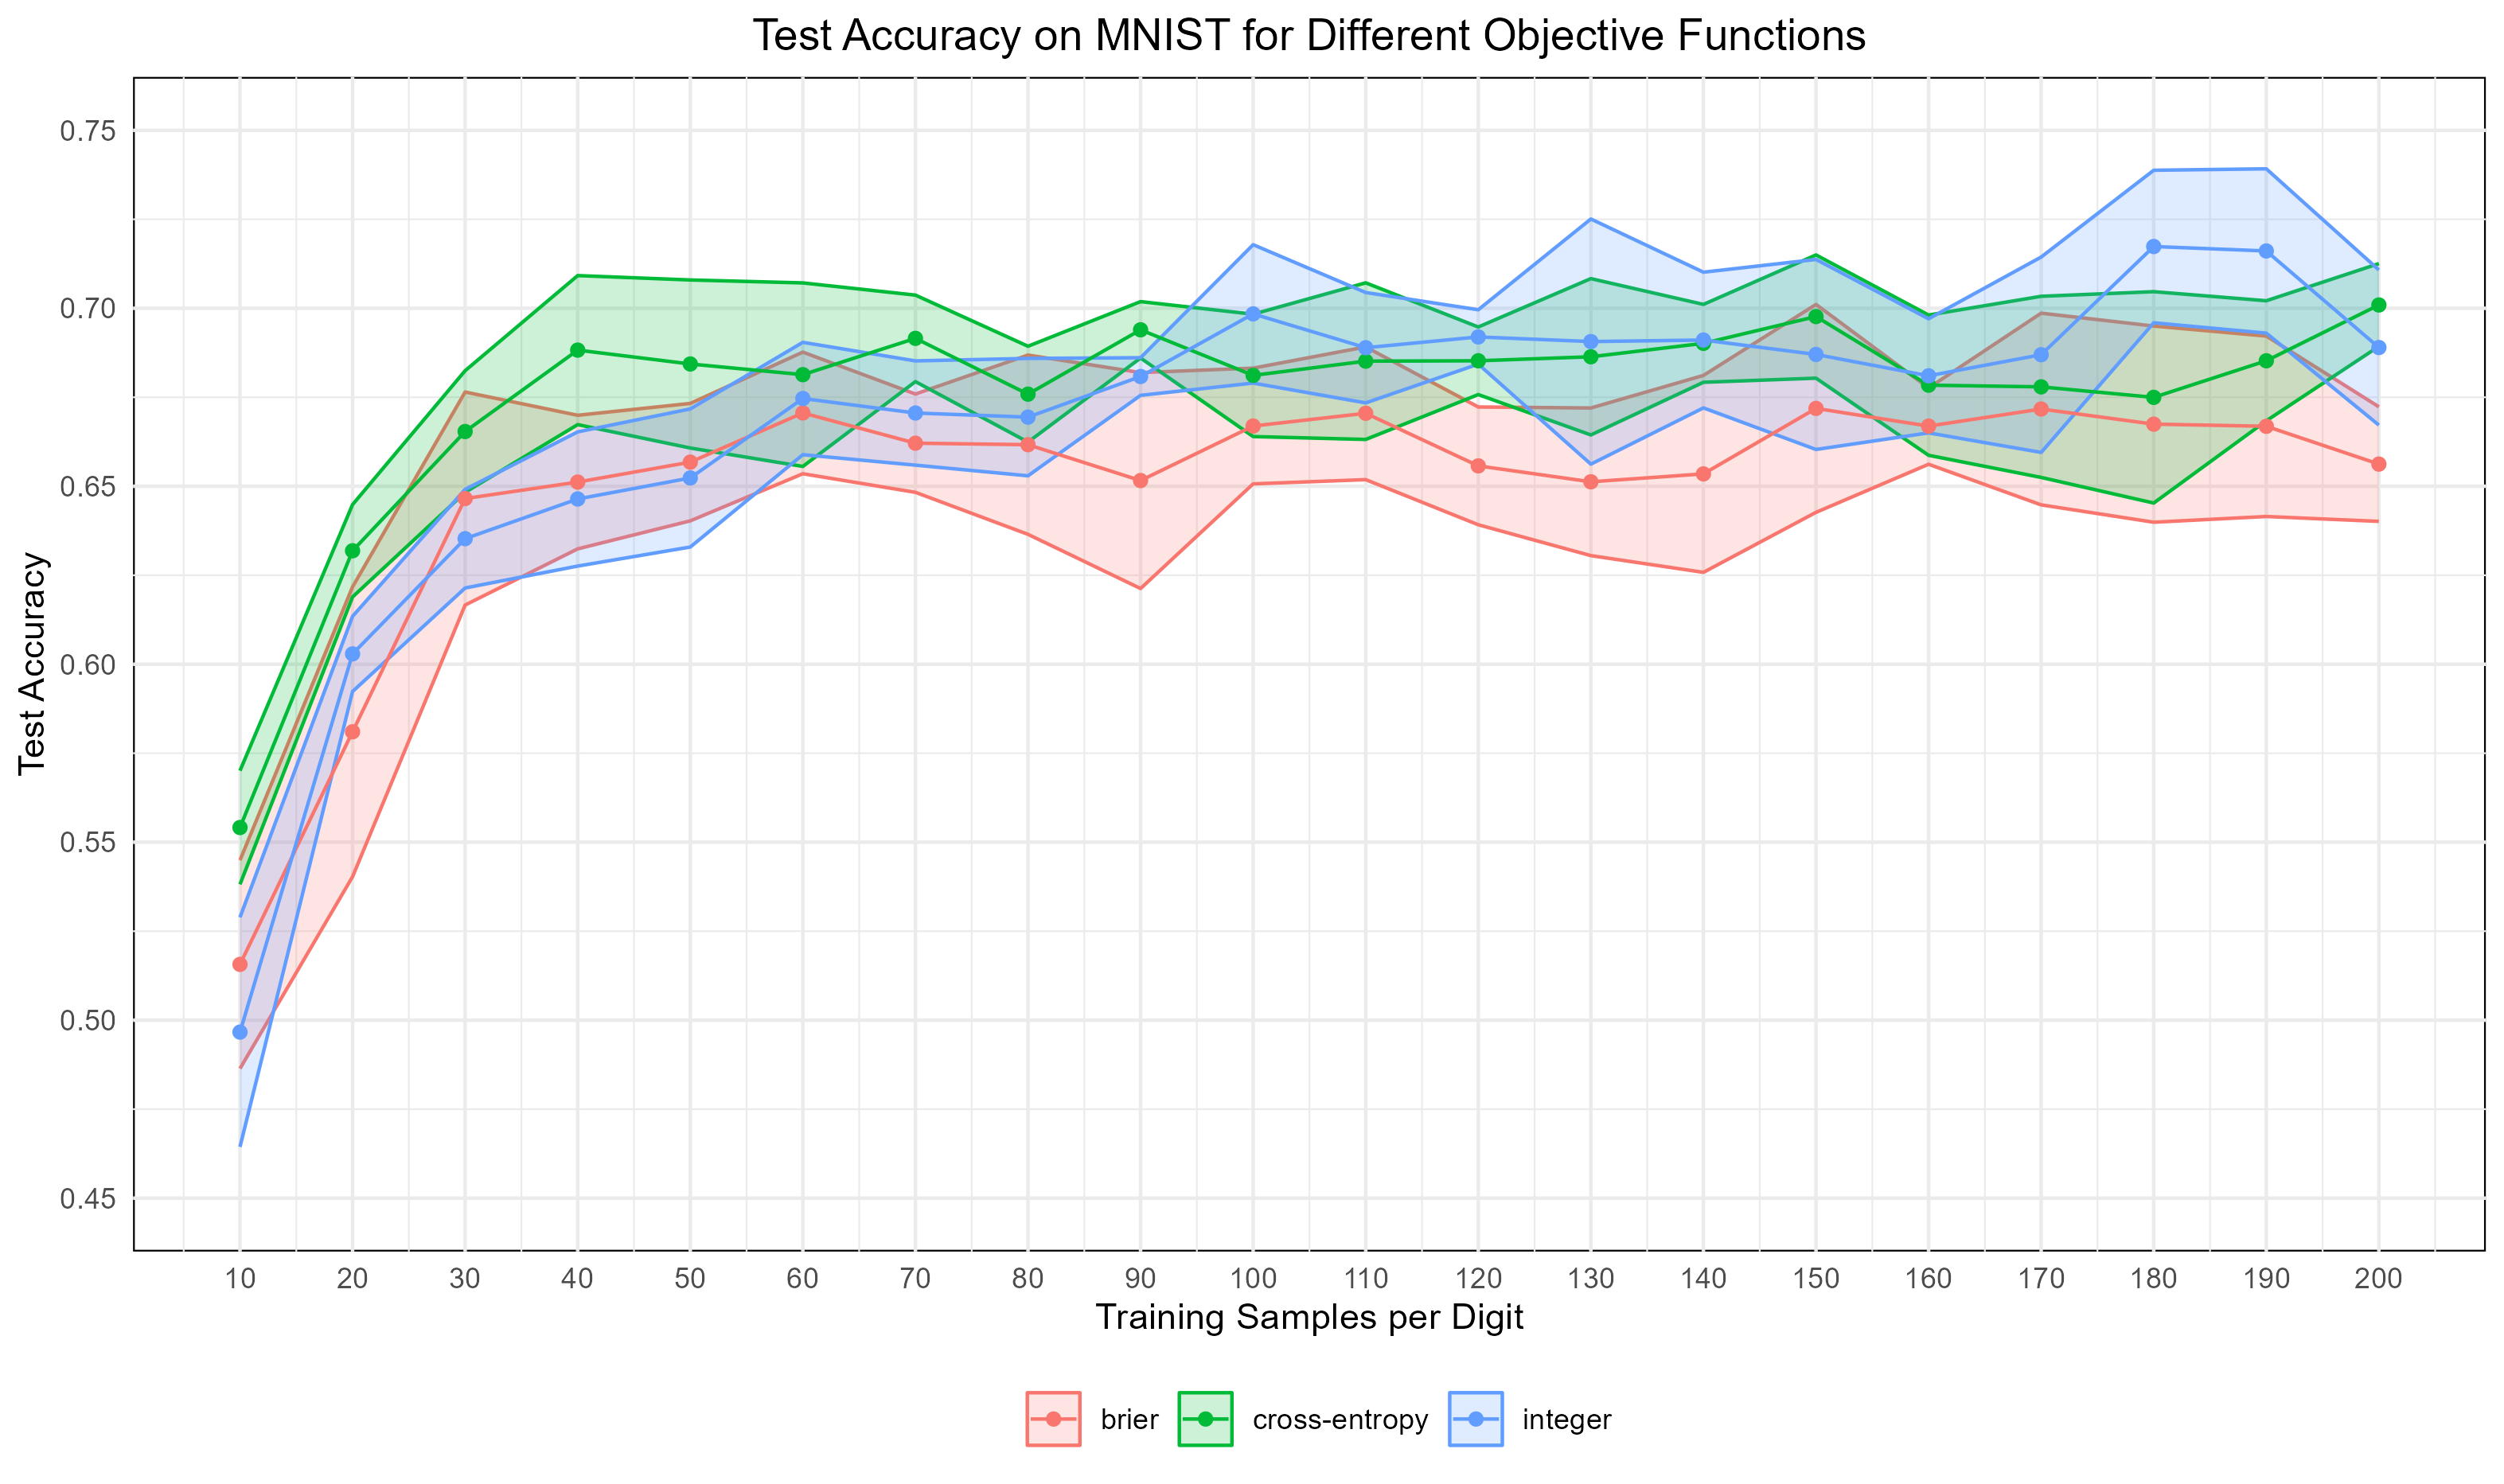
\includegraphics[width=1\linewidth]{Figures/SBT_COF.png}
    \caption{Testing accuracies for training a single batch on an increasing number of training samples. The x-axis shows the number of samples from each class in the batch and the y-axis shows the test accuracy. The results are for a BNN with a single hidden layer with 16 neurons using ILS with a time limit of 60 seconds. The batches are balanced, meaning that there is the same number of samples present from all classes. The testing accuracy is reported for 8000 samples, 800 from each class. The figure shows the mean accuracy of 5 runs as a line and the standard deviation of the accuracy as a shaded area around it. }
    \label{SBT_COF}
\end{figure}

\subsubsection{Testing the Effect of the Time Limit}
As a next step I investigate what the effect of the time limit is. Since the previous experiment showed that more training data give better results, there were signs that the effect took of as the amount of training data increased. The goal of this experiment is to investigate whether the results can get even better if the training is given more time. I test with a batch size of 2000 but now with different time limits ranging from 1 minute to 5 minutes. The mean accuracies can be seen in Table \ref{SBT_TETL_v2}, where it is evident that a time limit of 60 seconds was not enough. For all the objective functions, the accuracy increases as the time limit increases. The Brier objective function still cannot compete against the two other objective functions, which get very similar results. The maximum mean accuracy for this experiment is now 74.23 \%, an significant improven to the 71.73\% obtained before.   

\begin{center}
% latex table generated in R 4.2.2 by xtable 1.8-4 package
% Sun May 26 21:59:04 2024
\begin{table}[H]
\centering
\begin{tabular}{|c|c|c|c|c|c|}
  \hline
ObjectiveFunction & TL: 60 & TL: 120 & TL: 180 & TL: 240 & TL: 300 \\ 
  \hline
brier & 0.6562 & 0.6896 & 0.7063 & 0.7113 & 0.7149 \\ 
   \hline
cross-entropy & 0.7009 & 0.7202 & 0.7298 & 0.7360 & 0.7423 \\ 
   \hline
integer & 0.6890 & 0.7150 & 0.7340 & 0.7407 & 0.7413 \\ 
   \hline
\end{tabular}
\caption{The mean test accuracies on MNIST for different time limits. The results are obtained by training a 
            BNN on a single batch with 200 samples for each digit. The algorithm used is the ILS algorithm
            with perturbation size set to 25. The time limit is in seconds.} 
\label{SBT_TETL_v2}
\end{table}

\end{center}


\subsubsection{Comparing Different Network Structures}
I also want to test what effect the network architecture has. From the previous experiments, I found that increasing time limits and increasing amounts of data give better results. For this reason I use a time limit of 300 seconds and again a total batchsize of 2000 balanced sampled samples. Apart from the already tested network architecture with one layer with 16 neurons, I also try one with two layers, each with 16 neurons. I also try two larger networks with 128 neurons in each layer, where I test with one and two layers again. \\

\noindent From Table \ref{SBT_DNS}, it can be seen that the general pattern is that more neurons in the layers boost the accuracy significantly. For some reason, this does not seem to apply to the Brier objective function, where the accuracy decreases significantly. In deep learning, it often helps adding more layers, which is not the case here. The most likely reason for this is the fact that the amount of training data does not justify the second layer. This will be tested further in the next section. The cross-entropy objective function performs slightly better that the integer objective function in networks with only one hidden layer, but for networks with two hidden layers, the integer objective function outperforms the others. 
\begin{center}
% latex table generated in R 4.2.2 by xtable 1.8-4 package
% Sun May 26 21:59:08 2024
\begin{table}[H]
\centering
\begin{tabular}{|c|c|c|c|}
  \hline
Objective function & Hidden layers & 16 & 128 \\ 
  \hline
brier & One & 0.7149 & 0.5096 \\ 
   \hline
cross-entropy & One & 0.7423 & 0.8185 \\ 
   \hline
integer & One & 0.7413 & 0.8003 \\ 
   \hline
brier & Two & 0.5125 & 0.3795 \\ 
   \hline
cross-entropy & Two & 0.4844 & 0.6614 \\ 
   \hline
integer & Two & 0.5340 & 0.7284 \\ 
   \hline
\end{tabular}
\caption{The mean test accuracies on MNIST for different network structures. The results are obtained by training a BNN
            on a single batch with 2000 samples using the ILS algorithm with a time limit of 300 seconds.
            The columns indicates the width of the hidden layers} 
\label{SBT_DNS}
\end{table}

\end{center}



\subsubsection{Fine Tuning the Perturbation Size}

\noindent So far I have used a fixed parameter for the number of weights to change values for in the perturbation phase. The goal of this experiment is to see if there are room for improvement, i.e. if changing the perturbation size changes the results to the better. Ideally, all the results should be re-run with a different perturbation size to see if any of the conclusions drawn so far changes, but since each experiment takes a long time to run, this is not computationally feasible. Instead I take the configurations from the best results obtained so far, and use them to test if changing the perturbation size improves the results further. The best result obtained so far was with the cross entropy objective function and with a single hidden layer with 128 neurons. Since this is a relatively big network compared to some of the others, I also test changing the perturbation size for the network with 16 neurons in the hidden layer. The time limit is again 300 seconds. Besides from 25, I now try with perturbation sizes of 5, 10, 15, 20, 30, 35 and 40 as well. The results are given in Table \ref{SBT_FTPS}. For the small network architecture, the highest mean accuracy is achieved with a perturbation size of 40, whereas for the large network architecture it is with a perturbation size of 30. In general the results show that the perturbation size should not be too small. This is likely due to the reason that small perturbation sizes might mean that the solution return to the same local optima. This hyoerparameter experiment also shows that for the small network architecture tested in the first experiments, it is possible to achieve a even better accuracy of 75.95\%, again with only 2000 data samples. Further, with a larger network it is possible to achieve as high accuracy as 82.20\% using only this limited amount of data. 

\begin{center}
% latex table generated in R 4.2.2 by xtable 1.8-4 package
% Sun May 26 21:59:12 2024
\begin{table}[H]
\centering
\begin{tabular}{|c|c|c|c|}
  \hline
NeuronsHiddenLayer & PerturbationSize & Mean & SD \\ 
  \hline
16 &     5 & 0.7050 & 0.0085 \\ 
   \hline
16 &    10 & 0.7127 & 0.0153 \\ 
   \hline
16 &    15 & 0.7272 & 0.0240 \\ 
   \hline
16 &    20 & 0.7384 & 0.0207 \\ 
   \hline
16 &    25 & 0.7423 & 0.0074 \\ 
   \hline
16 &    30 & 0.7575 & 0.0129 \\ 
   \hline
16 &    35 & 0.7504 & 0.0149 \\ 
   \hline
16 &    40 & 0.7595 & 0.0153 \\ 
   \hline
128 &     5 & 0.8135 & 0.0041 \\ 
   \hline
128 &    10 & 0.8159 & 0.0018 \\ 
   \hline
128 &    15 & 0.8179 & 0.0042 \\ 
   \hline
128 &    20 & 0.8154 & 0.0037 \\ 
   \hline
128 &    25 & 0.8185 & 0.0058 \\ 
   \hline
128 &    30 & 0.8220 & 0.0054 \\ 
   \hline
128 &    35 & 0.8204 & 0.0040 \\ 
   \hline
128 &    40 & 0.8209 & 0.0076 \\ 
   \hline
\end{tabular}
\caption{The mean test accuracies on MNIST for two different networks with a single hidden layer.
            The results are obtained by training a BNN on a single batch with 2000 samples using the ILS
            algorithm with a time limit of 300 seconds. } 
\label{SBT_FTPS}
\end{table}

\end{center}


\subsection{Multiple Batch Training}
The goal of this section is to go a step further and train on more data using multiple batch training. The main motivation is that seeing more training data should help the model generalize better, but the important question is how to make use of more training data. From the first section it was already clear that using more data in a single batch setting requires more time. Instead of trying to continue to increase the batch size and train on a single batch, I instead want to train a model that sees many batches throughout the training. In this section I work with a overall time limit of 600 seconds. There are three algorithms that I test and compare against each other. I test two versions of Algorithm \ref{multiple_batches}, the first version is as the algorithm is presented with iterated improvement for each batch. The other version is with iterated local search for each batch. The goal of this is to investigate whether it helps seeing more data, but for less time, which is the case for the iterated improvement version, or if it is better to see less data, but find a better solution each time. These algorithms use early stopping to make sure that the solution returned is not too dependent on the last batch seen. \\

\noindent The third algorithm is Algorithm \ref{multiple_batches_v2}, where less moves are committed, but every move should generalize better, as a move is only committed if it improves the solution across several batches. The main question is, whether this algorithm can compete against the others and whether it is too slow compared to the others. In this section I do not use balanced training and test sets anymore. MNIST is not uniformly distributed and the main reason for using balanced training and test set was to make fair comparisons against existing literature. I still train on a BNN and I use a batch size of 1,000. Whenever I use early stopping I take 20 \% of the training set, 12,000 samples, and use as validation set. For iterated improvement I calculate the validation accuracy after every fourth batch, where for ILS I do it after every single batch. I test the same four network architectures as earlier. The accuracies are calculated on the entire test set of 10,000 samples. \\

\noindent The first experiment in this section is again to test objective functions against each other and to see if they perform differently under different circumstances. For this I test the three different objective functions on four different network structures and with all three algorithms. Afterwards I investigate whether the sporadic local search has any positive impact by testing the $bp$ parameter. 

\subsubsection{Comparing Objective Functions}
The goal of the first experiment is to see what objective function and algorithm work best. I use the settings specified above. For the ILS version, I let each ILS phase take 5 seconds and set $ps=25$. For all the algorithms I set $bp=0.2$. I set $updateStart=1$, $updateEnd=15$ and $updateIncrease=10$. Table \ref{MBT} presents the mean accuracies. For the networks with 16 neurons in each hidden layer, it is the case for all configurations, that the single layer version performs best. Further, for the network with 16 neurons and a single hidden layer, the Brier objective function now perform almost as good as the cross entropy in two of the algorithms and for the aggregation algorithm even sligtly better. With two hidden layers, each with 16 neurons, the Brier score objective function clearly outperforms the other objective functions. 

\noindent When the network size increases, the results are different. For both networks with a single hidden layer and two hidden layers each with 128 neurons, the aggregation algorithm is the best. What is more surprising is that the integer objective function now is best in all cases except for the one layer case with the aggregation algorithm. With two hidden layers, the integer objective function clearly outperforms the other objective functions. One of the reasons why this objective function is better might be due to the fact that it is much faster. To see this, look at Table \ref{MBT_II}, where I take a deeper look into the iterated improvement version of Algorithm \ref{multiple_batches}. Specifically, I take a look at how many batches the different objective functions iterate through within the time limit of 600 seconds. Here it is clear, that for all the configurations, the integer objective function iterates through more batches and as a results see more data. \\

\noindent I also take a look at the number of moves made per batch. As this number is expected to decrease as the number of batches increase, I also present the number for the first 30 batches. In both cases, the pattern is the same. For the integer objective function, less moves are made. This suggests that the number of batches seen is not higher only because the integer objective function is faster in computation time, but also because less moves are made in each iteration. This is not necessarily a bad thing. The more moves that are made at each iteration, the more the current solution depends on the current batch. As a result, the gap between training accuracy and validation or test accuracy might be larger for the objective functions that make more moves based on the current batch. This is especially evident from Figure \ref{MBT_II_INTEGER}, \ref{MBT_II_BRIER} and \ref{MBT_II_CROSS_ENTROPY_FUNCTION} that plots the training accuracies and the validation accuracies for each of the three objective functions. The plots are based on iterated improvement algorithm and the network architecture with two hidden layers with 128 neurons each. The gap is quite small for the integer objective function compared to the Brier and cross entropy objective functions. \\

\noindent These are possible reasons why the integer objective function is better, but they do not necessarily explain why it is only better for larger networks. However, this is probably due to the definition of the objective function, that does not work with probability or probability distributions, but with maximizing the margins. For small networks it seem that this is not possible in the same way as with larger networks, where the integer objective function is better than the other objective functions in most cases. 

\begin{center}
% latex table generated in R 4.2.2 by xtable 1.8-4 package
% Sat May 25 12:43:53 2024
\begin{table}[H]
\centering
\begin{tabular}{|c|c|c|c|c|}
  \hline
Objective function & Hidden layers & Algorithm & 16 & 128 \\ 
  \hline
brier & One & Iterated Improvement & 0.8205 & 0.8479 \\ 
   \hline
brier & One & Aggregation Algorithm & 0.8491 & 0.8858 \\ 
   \hline
brier & One & Iterated Local Search & 0.7938 & 0.8499 \\ 
   \hline
cross-entropy & One & Iterated Improvement & 0.8223 & 0.8432 \\ 
   \hline
cross-entropy & One & Aggregation Algorithm & 0.8478 & 0.8655 \\ 
   \hline
cross-entropy & One & Iterated Local Search & 0.7992 & 0.8416 \\ 
   \hline
integer & One & Iterated Improvement & 0.8038 & 0.8668 \\ 
   \hline
integer & One & Aggregation Algorithm & 0.7919 & 0.8781 \\ 
   \hline
integer & One & Iterated Local Search & 0.7887 & 0.8632 \\ 
   \hline
brier & Two & Iterated Improvement & 0.7852 & 0.7005 \\ 
   \hline
brier & Two & Aggregation Algorithm & 0.8265 & 0.8454 \\ 
   \hline
brier & Two & Iterated Local Search & 0.7458 & 0.7191 \\ 
   \hline
cross-entropy & Two & Iterated Improvement & 0.7390 & 0.6736 \\ 
   \hline
cross-entropy & Two & Aggregation Algorithm & 0.6936 & 0.7997 \\ 
   \hline
cross-entropy & Two & Iterated Local Search & 0.7048 & 0.6986 \\ 
   \hline
integer & Two & Iterated Improvement & 0.5677 & 0.8878 \\ 
   \hline
integer & Two & Aggregation Algorithm & 0.4416 & 0.9153 \\ 
   \hline
integer & Two & Iterated Local Search & 0.7095 & 0.8766 \\ 
   \hline
\end{tabular}
\caption{The mean test accuracies on MNIST for different network structures and algorithms. The network is a
            BNN trained with a time limit of 600 seconds. Iterated Improvement and Iterated Local Search refers to
            Algorithm 4, and here early stopping is used. The validation dataset is 12,000 samples and for
            II, the validation accuracy is calculated every fourth batch, whereas for ILS, it is after every batch.
            The solution with the highest validation accuracy is returned. I set bp equal to 0.2 and ps to 25.
            Each ILS phase is allowed to run for 5 seconds. 
            For the Aggregation Algorithm, I do not use early stopping, but return the solution at the end. The parameters
            updateStart, updateEnd and updateIncrease are set to 1, 15 and 10 respectively. For all the algorithms
            a batch size of 1000 is used. } 
\label{MBT}
\end{table}

\end{center}


\begin{center}
% latex table generated in R 4.2.2 by xtable 1.8-4 package
% Sun Jun  2 21:10:30 2024
\begin{table}[!tb]
\centering
\begin{tabular}{|c|c|c|c|c|c|}
  \hline
Objective function & Hidden layers & Mean & MeanBatches & MeanMoves & MeanMoves30 \\ 
  \hline
brier & 16 & 0.8205 & 427.20 & 213.0588 & 236.5333 \\ 
   \hline
cross-entropy & 16 & 0.8223 & 475.20 & 174.5439 & 217.9800 \\ 
   \hline
integer & 16 & 0.8038 & 594.20 & 107.2392 & 115.9400 \\ 
   \hline
brier & 16-16 & 0.7852 & 392.80 & 179.3991 & 181.5333 \\ 
   \hline
cross-entropy & 16-16 & 0.7390 & 394.60 & 183.8709 & 178.2067 \\ 
   \hline
integer & 16-16 & 0.5677 & 591.60 & 66.0823 & 84.8200 \\ 
   \hline
brier & 128 & 0.8479 & 45.80 & 4205.4210 & 4191.3800 \\ 
   \hline
cross-entropy & 128 & 0.8432 & 62.60 & 2854.2981 & 2988.1267 \\ 
   \hline
integer & 128 & 0.8668 & 147.80 & 993.4502 & 1158.5133 \\ 
   \hline
brier & 128-128 & 0.7005 & 48.40 & 2542.8706 & 2049.0067 \\ 
   \hline
cross-entropy & 128-128 & 0.6736 & 47.00 & 2579.0009 & 2537.3467 \\ 
   \hline
integer & 128-128 & 0.8878 & 110.80 & 887.7500 & 935.8800 \\ 
   \hline
\end{tabular}
\caption{\small{\textbf{Summary statistics for the iterated improvement version of Algorithm 4. 
            'MeanBatches' is the average number of batches seen, MeanMoves' is the average number of moves made per batch,
            and MeanMoves30 is the average number of moves made per batch in the first 30 batches.}}} 
\label{MBT_II}
\end{table}

\end{center}


\begin{figure}[H]
    \centering
    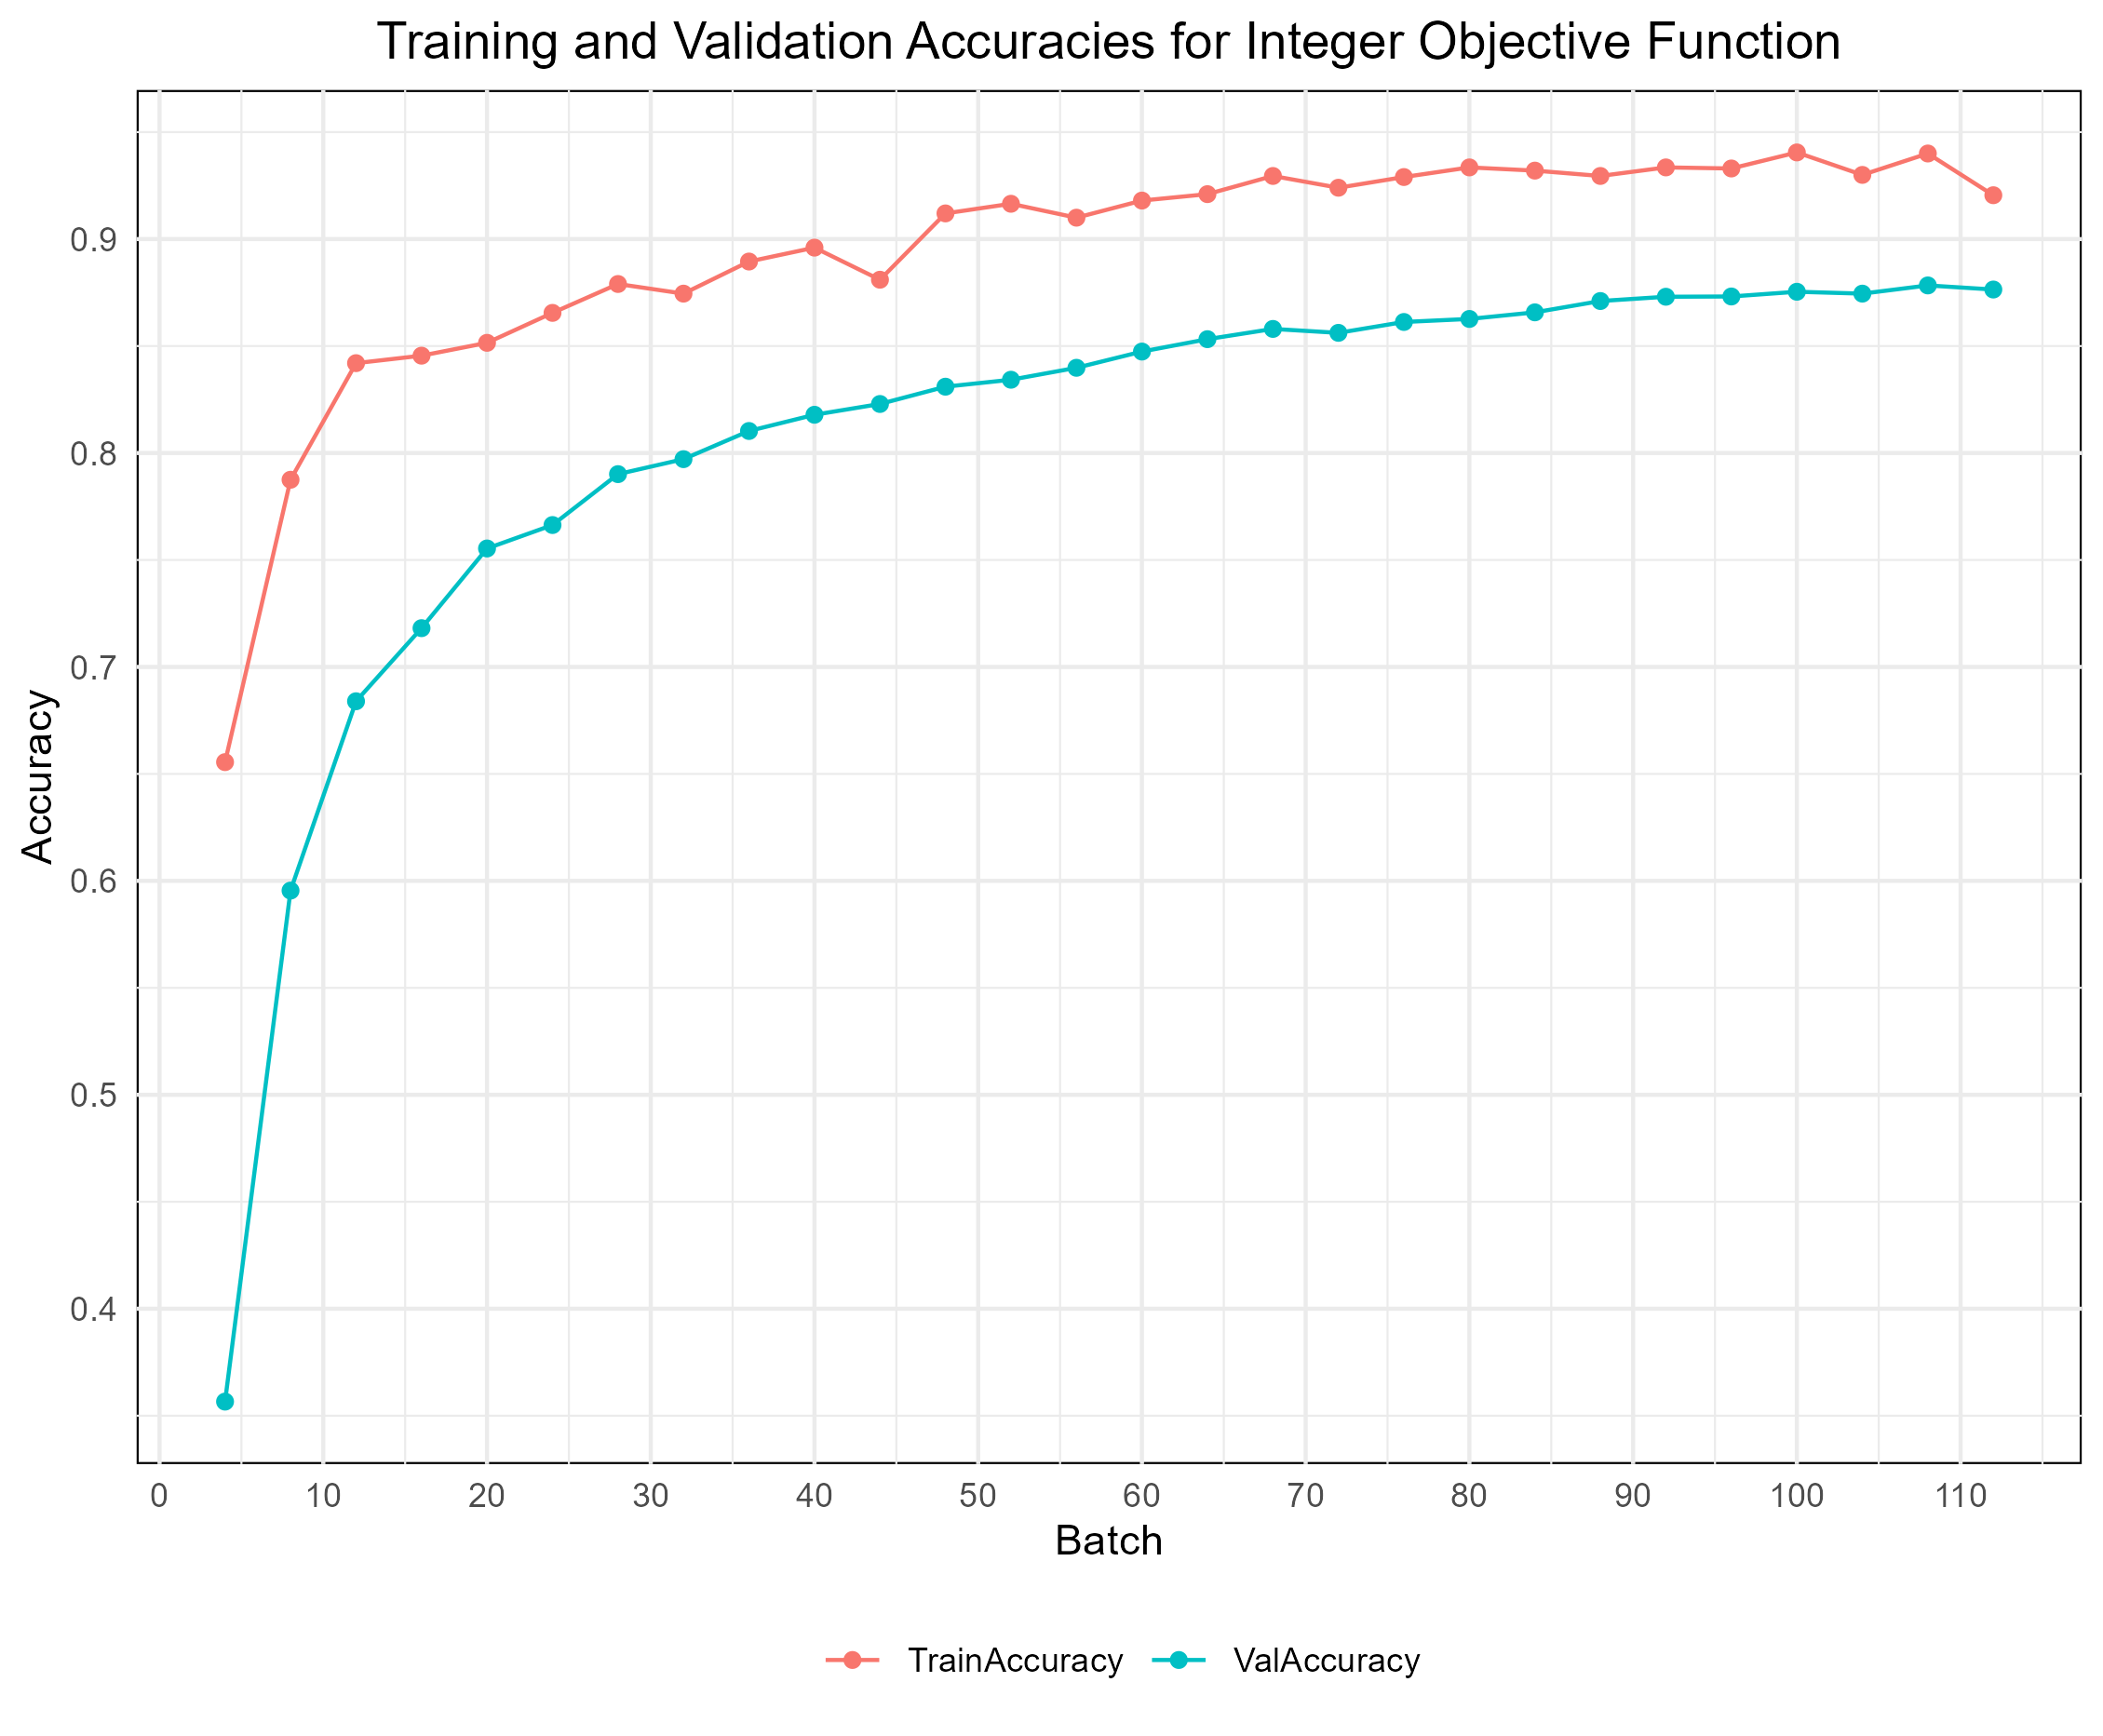
\includegraphics[width=1\linewidth]{Figures/MBT_II_INTEGER.png}
    \caption{Training and validation accuracies for the iterated improvement algorithm with the integer objective function. The network structure is with two hidden layers, each with 128 neurons in each. As such, the plot is for the bottom row of Table \ref{MBT_II}.}
    \label{MBT_II_INTEGER}
\end{figure}

\begin{figure}[H]
    \centering
    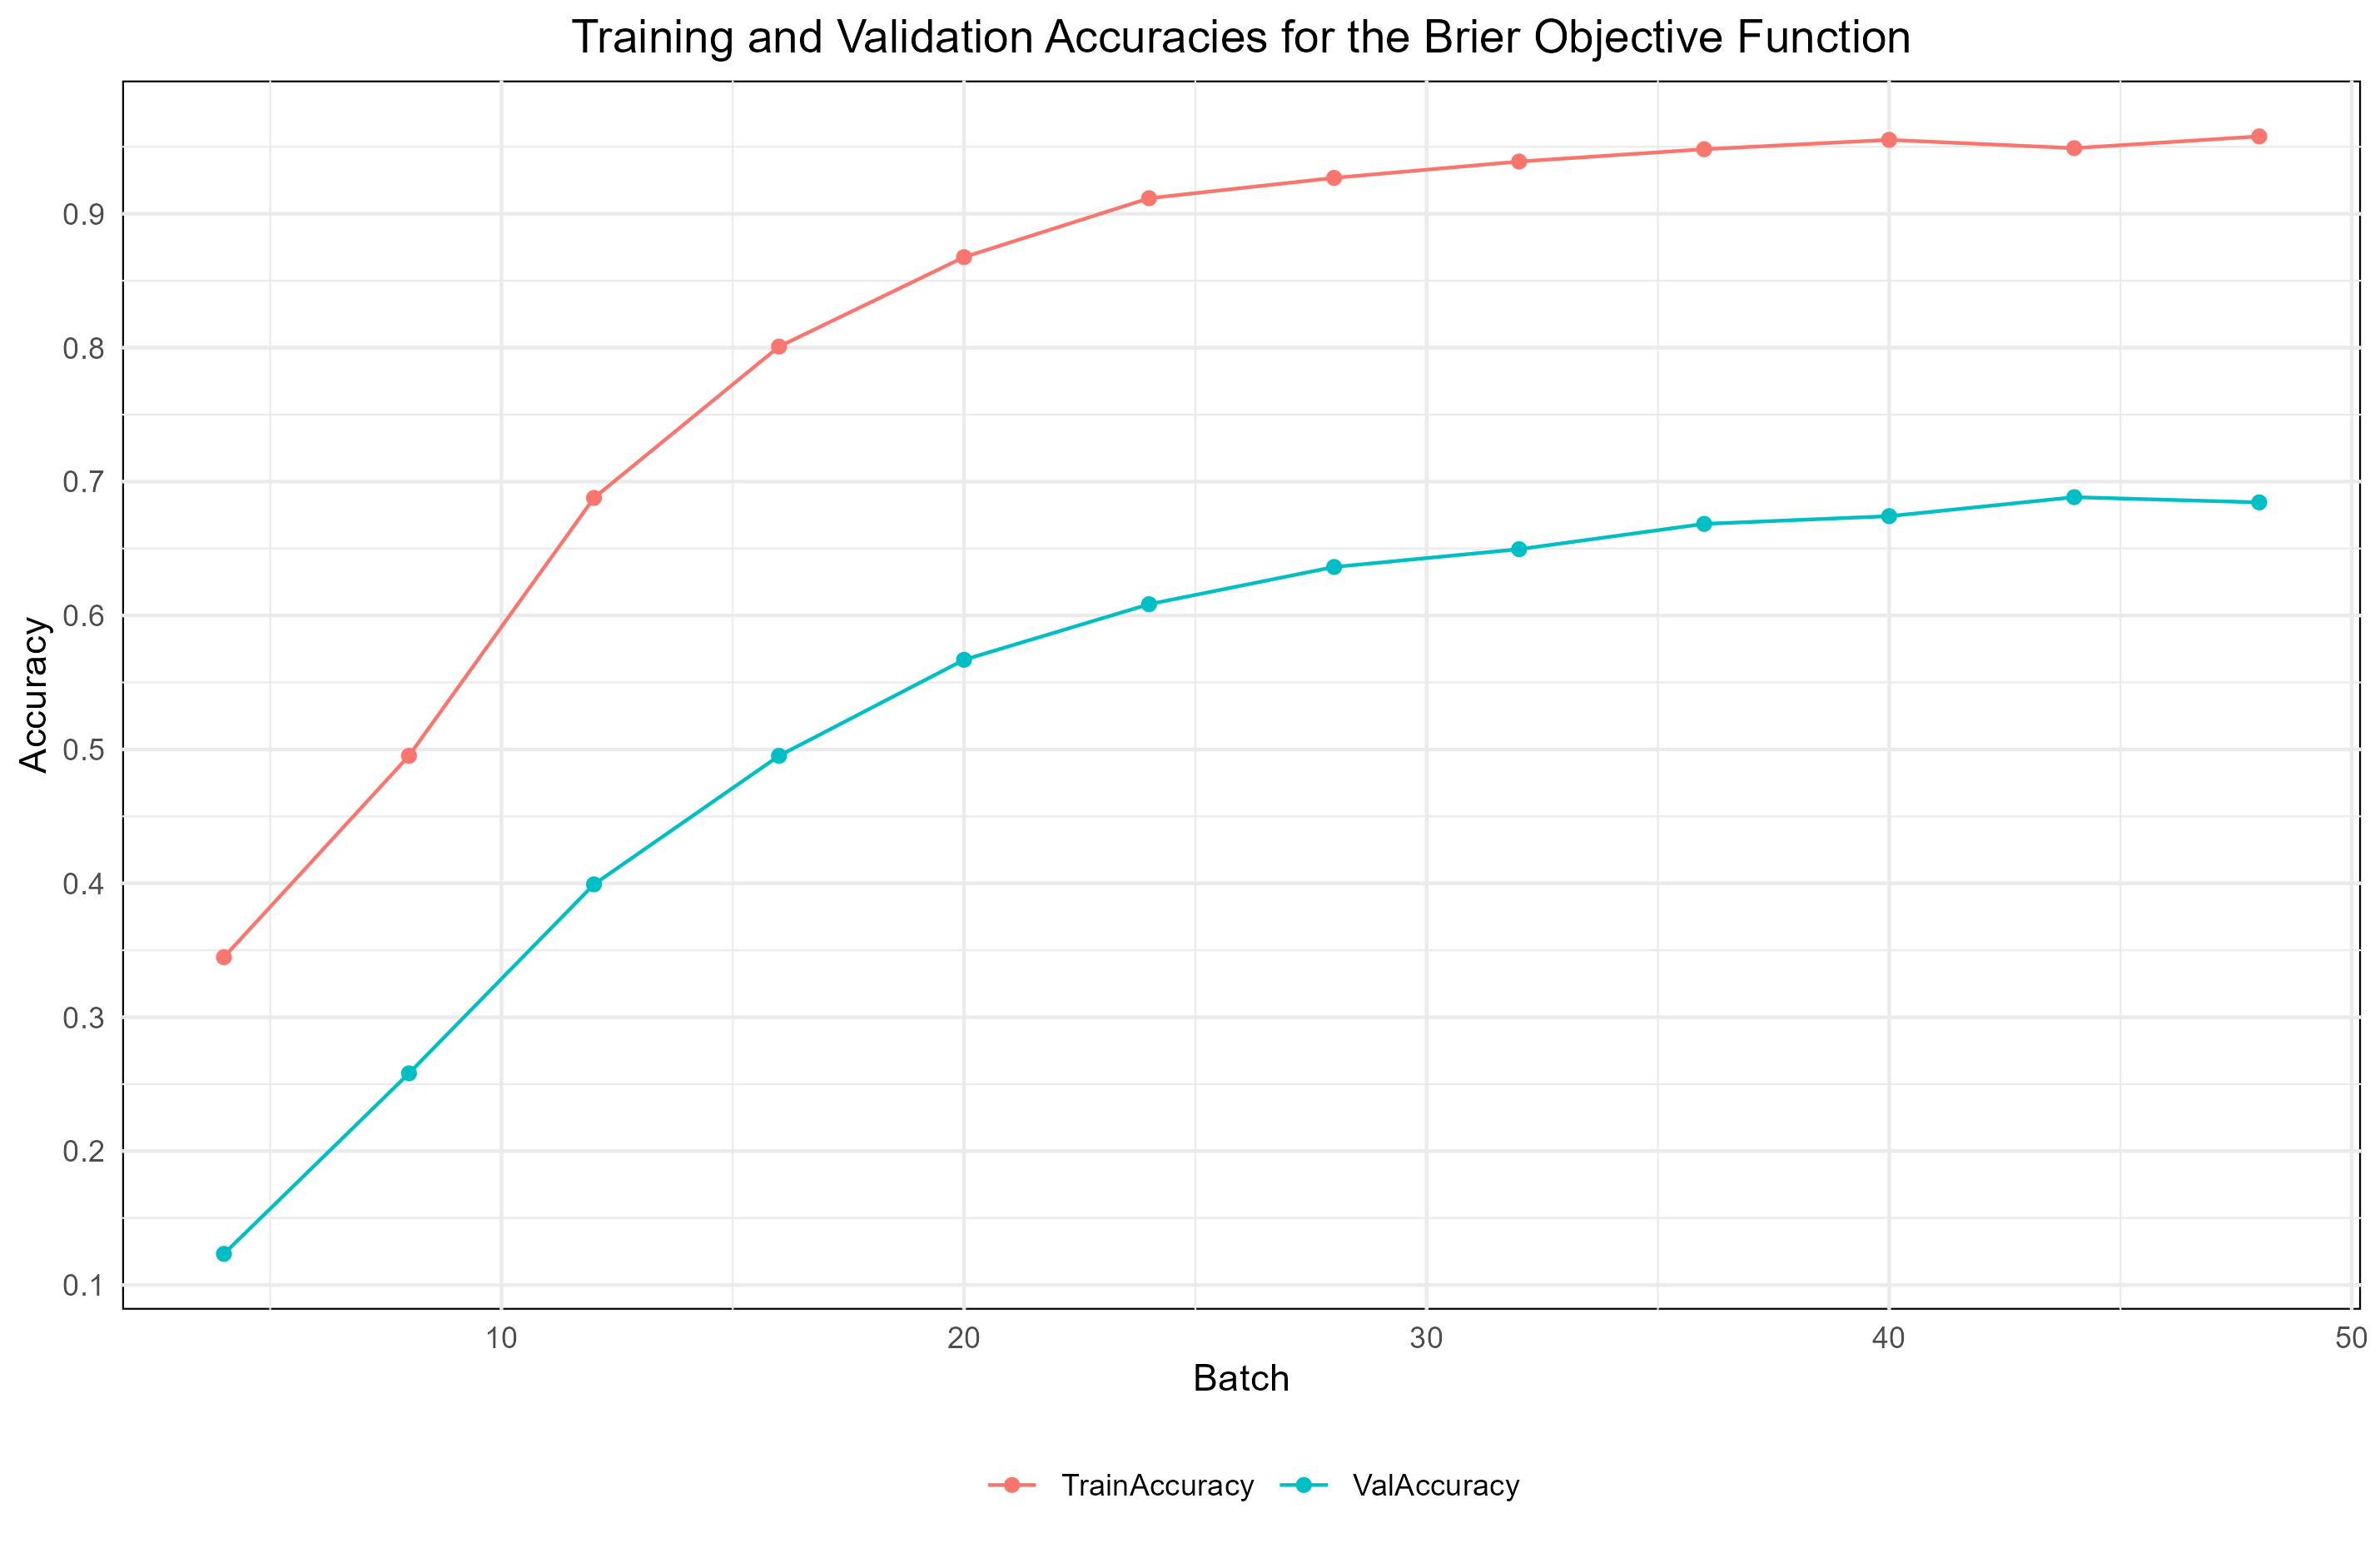
\includegraphics[width=1\linewidth]{Figures/MBT_II_BRIER.png}
    \caption{Training and validation accuracies for the iterated improvement algorithm with the Brier objective function. The network structure is with two hidden layers, each with 128 neurons in each. As such, the plot is for the third last row of Table \ref{MBT_II}.}
    \label{MBT_II_BRIER}
\end{figure}

\begin{figure}[H]
    \centering
    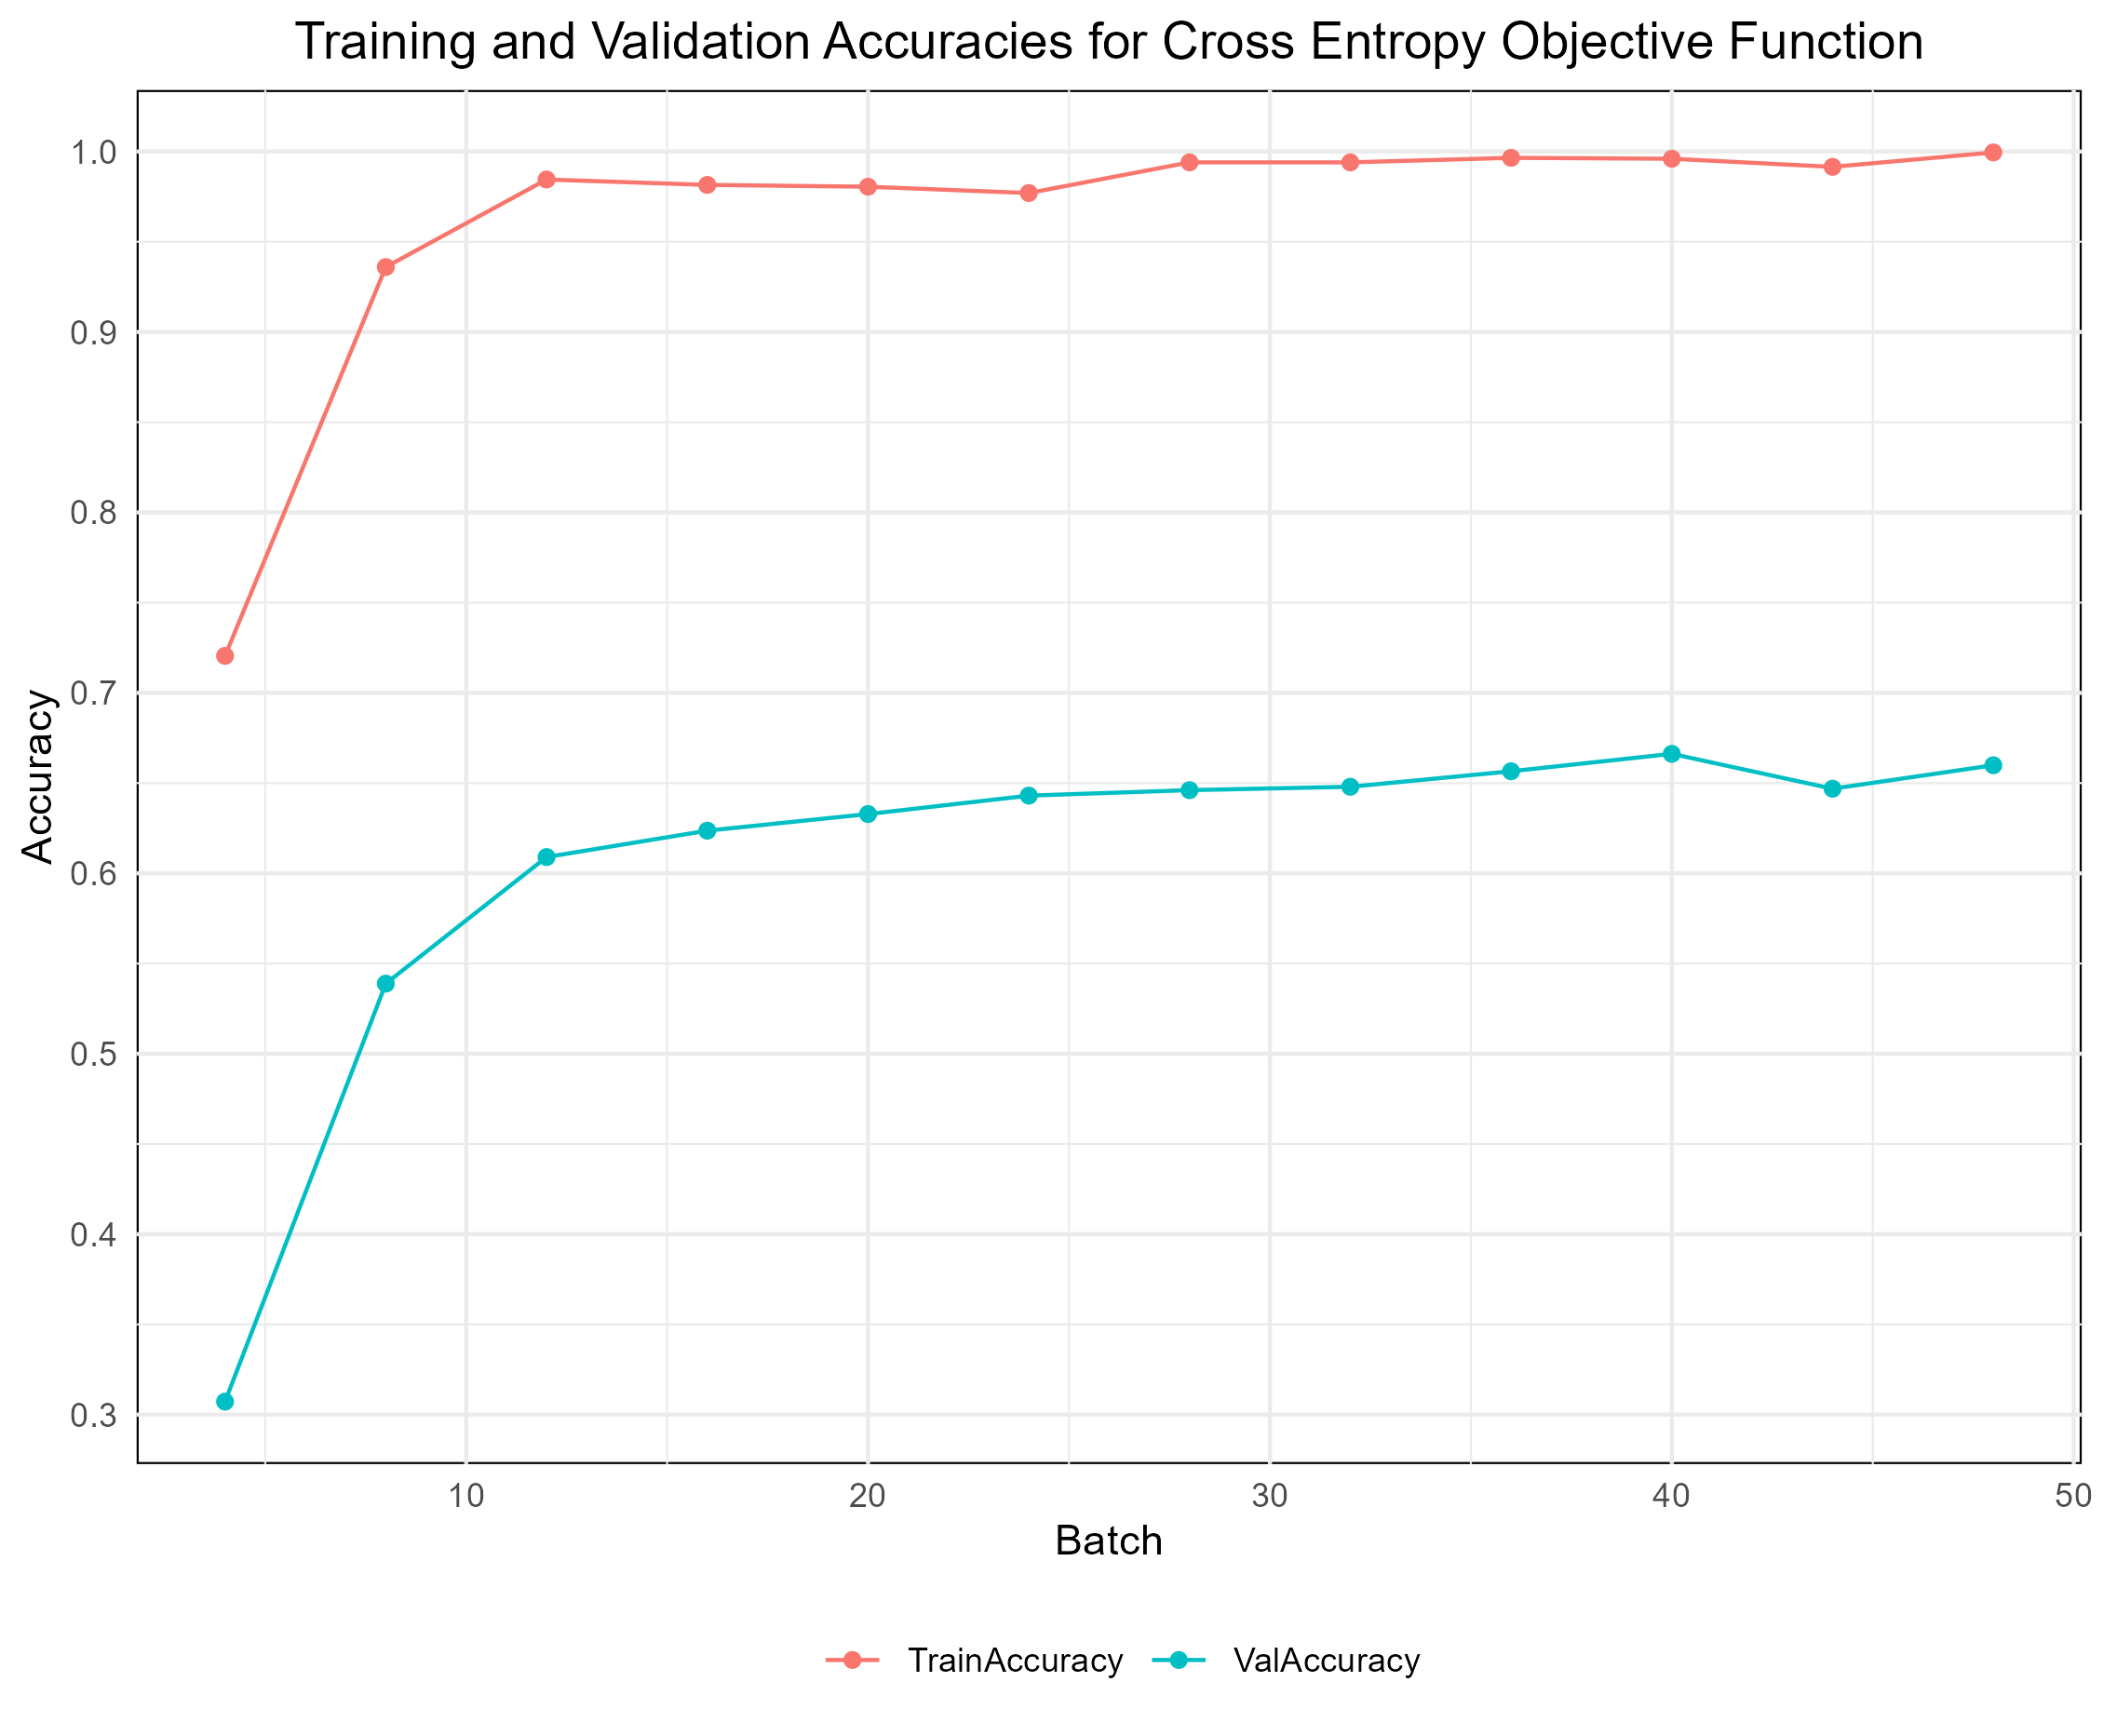
\includegraphics[width=1\linewidth]{Figures/MBT_II_CROSS_ENTROPY.png}
    \caption{Training and validation accuracies for the iterated improvement algorithm with the cross entropy objective function. The network structure is with two hidden layers, each with 128 neurons in each. As such, the plot is for the second last row of Table \ref{MBT_II}. }
    \label{MBT_II_CROSS_ENTROPY_FUNCTION}
\end{figure}




\subsubsection{Testing the Effect of Sporadic Local Search}
For all the three algorithms I used sporadic local search, where the parameter $bp$ determines the probability that a weight is part of the search in that iteration. Until now I used $bp=0.2$, but now I change the value of this to see how important it is and if it has any affect at all. Notice that $bp=1$ corresponds to not using sporadic local search, as here all weights are subject to change in each iteration. The hope is that using sporadic local search would improve the ability of the model to generalize by being less dependent on the current batch. For the aggregation algorithm, this is not necessarily true, as the algorithm here do not make moves based on a single batch. Instead of $bp=0.2$ I now try with 0.1, 0.3, 0.4, 0.5 and 1 as values. I choose the best configuration from the previous experiment, so I use a network architecture with 2 hidden layers, each with 128 neurons and I use the integer objective function. The mean test accuracies can be seen in Table \ref{MBT_FTBP}, where the results are somewhat disappointing. For ILS and iterated improvement, the test accuracies are better with no use of sporadic local search and for the aggregation algorithm the results are very similar across different values of $bp$, so there seems to be no positive effect of using sporadic local search. 


\begin{center}
% latex table generated in R 4.2.2 by xtable 1.8-4 package
% Sun Jun  2 21:27:35 2024
\begin{table}[!tb]
\centering
\begin{tabular}{|c|c|c|c|}
  \hline
Algorithm & BP & Mean & SD \\ 
  \hline
Iterated Improvement & 0.1 & 0.8825 & 0.0030 \\ 
   \hline
Iterated Improvement & 0.2 & 0.8878 & 0.0033 \\ 
   \hline
Iterated Improvement & 0.3 & 0.8917 & 0.0039 \\ 
   \hline
Iterated Improvement & 0.4 & 0.8896 & 0.0051 \\ 
   \hline
Iterated Improvement & 0.5 & 0.8917 & 0.0033 \\ 
   \hline
Iterated Improvement & 1.0 & 0.8976 & 0.0030 \\ 
   \hline
Aggregation Algorithm & 0.1 & 0.9130 & 0.0030 \\ 
   \hline
Aggregation Algorithm & 0.2 & 0.9153 & 0.0025 \\ 
   \hline
Aggregation Algorithm & 0.3 & 0.9125 & 0.0009 \\ 
   \hline
Aggregation Algorithm & 0.4 & 0.9132 & 0.0013 \\ 
   \hline
Aggregation Algorithm & 0.5 & 0.9131 & 0.0032 \\ 
   \hline
Aggregation Algorithm & 1.0 & 0.9147 & 0.0032 \\ 
   \hline
Iterated Local Search & 0.1 & 0.8564 & 0.0054 \\ 
   \hline
Iterated Local Search & 0.2 & 0.8766 & 0.0050 \\ 
   \hline
Iterated Local Search & 0.3 & 0.8806 & 0.0039 \\ 
   \hline
Iterated Local Search & 0.4 & 0.8826 & 0.0031 \\ 
   \hline
Iterated Local Search & 0.5 & 0.8844 & 0.0038 \\ 
   \hline
Iterated Local Search & 1.0 & 0.8939 & 0.0033 \\ 
   \hline
\end{tabular}
\caption{\small{\textbf{The mean test accuracies on MNIST for three different algorithms with different values of bp.
            The results are obtained by training a BNN for a time limit of 600 seconds. For II, k=4, for
            ILS, k=1 and each ILS phase runs for 5 seconds with a perturbation size of 25. For AA updateStart, updateEnd
            and updateIncrease are 1, 15 and 10 respectively.}}} 
\label{MBT_FTBP}
\end{table}

\end{center}



\subsection{Ternary Neural Networks}
\noindent In a TNN, the weights can also be zero, which increases the capacity of the model. As a result the solution space gets bigger and the delta evaluation takes more time. When considering a move in a BNN, there is only one other possible value. For a TNN, two other values need to be considered. For this reason, I expect that training a TNN takes longer time, but the hope is that, as the model has a larger capacity, it will be able to give higher accuracies as well. The goal of this section is to explore TNNs. At first I will test the effect of adding a regularization parameter, as introduced in section 5.3.5. Secondly, I will investigate if it takes longer to train a TNN compared to a BNN. The results in these sections are comparable to existing literature on training NNs using MIP, so here I again use balanced training and test sets and train on a single batch.


\subsubsection{Testing the Effect of a Regularization Parameter}

I start by testing the effect of the regularization parameter by testing different values. I train on a single batch, with 2000 samples and the network has a single hidden layer with 16 neurons, so the most comparable results obtained so far are those from the Single Batch Training section. I try with all 3 objective functions and different values of the regularization parameter. Whenever this parameter is equal to zero it corresponds to training a TNN without any additional regularization term. From Table \ref{SBT_TETL_v2}, the results for training a BNN with the same settings are given. Here, for a time limit of 300 seconds, the accuracies were 71.49 \%, 74.23 \% and 74.13 \% for the Brier, cross entropy and integer objective function respectively. From Table \ref{TNN_COF}, it can be seen that whenever no regularization parameter is added, the mean accuracies already increase for the Brier and cross entropy objective functions, where for the integer the accuracy decrease compared to BNN. \\

\noindent In Table \ref{TNN_COF}, the 'Connections' column show the average number of active connections, i.e. the weights whose value are not 0. The same value of the regularization parameter does not seem to have the same effect across objective functions. It seems that the integer objective function needs higher values of the regularization parameter compared to the other objective functions. This is related to the definition of the objective function and in particular the range of the objective function value. For the Brier objective function, there seems to be a positive effect of adding a regularization parameter of around 1.0, so I run another experiment to finetune this further. From Table \ref{TNN_REG_BRIER}, it seems to be the case that a value between 1.5 and 2.5 gives the highest accuracies with a maximum mean accuracy of 76.22 \% for a value of 2. For this value, the average number of active connections is 572. The total number of connections in the network is $784 \cdot 16 + 16 \cdot 10 = 12,704$, so it is less than 5\% of the connections that are actually active. \\

\noindent For the cross entropy function, at first sight looking at Table \ref{TNN_COF}, there is no value of the regularization parameter that gives higher accuracy, but a value of 1.0 comes close, so again I try another experiment to finetune further. Table \ref{TNN_REG_CS} shows indeed that it was possible to find values of the regularization parameter, that gave higher accuracies. The maximum mean accuracy here os 76.65 \%, but this time with a value of 4.0 for the regularization parameter. It is interesting that the average number of active connections in this case is 574, which is very close to the same number for the Brier objective function. For the integer objective function, there does not seem to be a positive effect, neither in Table \ref{TNN_COF} or \ref{TNN_REG_INT}, where I tried with more values. \\

\noindent It should be mentioned, that this finetuning was with respect to the specific settings used here. By the way the objective function terms are defined it is highly likely that changing either the number of connections in the network, i.e. the network architecture or the number of samples in the batch, then a new finetuning is possible. Thus, it is not expected that these values of the regularization parameter generalize well to other settings, but nevertheless the results show that for the Brier and cross entropy objective functions, there is something to be gained when regularizing the network. For the integer objective function, regularization did not seem to have any positive influence. 


\begin{center}
% latex table generated in R 4.2.2 by xtable 1.8-4 package
% Sat Jun  1 15:52:08 2024
\begin{table}[!tb]
\centering
\begin{tabular}{|c|c|c|c|c|c|}
  \hline
Reg & ObjectiveFunc & Mean & SD & Connections & LocalOptimas \\ 
  \hline
 0.00000 & brier & 0.7264 & 0.0209 & 8813 &  98 \\ 
   \hline
 0.00001 & brier & 0.7057 & 0.0124 & 5053 &  59 \\ 
   \hline
 0.00010 & brier & 0.7100 & 0.0095 & 4928 &  60 \\ 
   \hline
 0.00100 & brier & 0.7143 & 0.0137 & 4785 &  68 \\ 
   \hline
 0.01000 & brier & 0.7025 & 0.0047 & 4447 &  82 \\ 
   \hline
 0.10000 & brier & 0.7088 & 0.0177 & 3776 & 106 \\ 
   \hline
 1.00000 & brier & 0.7492 & 0.0089 & 1348 & 116 \\ 
   \hline
10.00000 & brier & 0.6811 & 0.0202 &  393 &  62 \\ 
   \hline
 0.00000 & cross-entropy & 0.7471 & 0.0158 & 8774 & 117 \\ 
   \hline
 0.00001 & cross-entropy & 0.7270 & 0.0076 & 5011 &  69 \\ 
   \hline
 0.00010 & cross-entropy & 0.7283 & 0.0175 & 4984 &  69 \\ 
   \hline
 0.00100 & cross-entropy & 0.7251 & 0.0095 & 4923 &  74 \\ 
   \hline
 0.01000 & cross-entropy & 0.7242 & 0.0093 & 4743 &  78 \\ 
   \hline
 0.10000 & cross-entropy & 0.7346 & 0.0128 & 4093 & 105 \\ 
   \hline
 1.00000 & cross-entropy & 0.7446 & 0.0112 & 2349 & 130 \\ 
   \hline
10.00000 & cross-entropy & 0.7359 & 0.0123 &  228 &  65 \\ 
   \hline
 0.00000 & integer & 0.7315 & 0.0174 & 8690 & 235 \\ 
   \hline
 0.00001 & integer & 0.7120 & 0.0143 & 4462 & 130 \\ 
   \hline
 0.00010 & integer & 0.7134 & 0.0139 & 4461 & 131 \\ 
   \hline
 0.00100 & integer & 0.7121 & 0.0142 & 4462 & 130 \\ 
   \hline
 0.01000 & integer & 0.7127 & 0.0139 & 4462 & 130 \\ 
   \hline
 0.10000 & integer & 0.7140 & 0.0138 & 4462 & 131 \\ 
   \hline
 1.00000 & integer & 0.7214 & 0.0153 & 4166 & 127 \\ 
   \hline
10.00000 & integer & 0.7257 & 0.0196 & 1212 & 142 \\ 
   \hline
\end{tabular}
\caption{\small{\textbf{Summary statistics for single batch training of a TNN with 2000 samples. 
          The network trained has a single hidden layer with 16 neurons and is trained for
          300 seconds.}}} 
\label{TNN_COF}
\end{table}

\end{center}

\begin{center}
% latex table generated in R 4.2.2 by xtable 1.8-4 package
% Sat Jun  1 17:01:34 2024
\begin{table}[!tb]
\centering
\begin{tabular}{|c|c|c|c|c|c|}
  \hline
Reg & ObjectiveFunc & Mean & SD & Connections & LocalOptimas \\ 
  \hline
0.00 & brier & 0.7264 & 0.0209 & 8813 &  98 \\ 
   \hline
0.50 & brier & 0.7308 & 0.0099 & 2349 & 123 \\ 
   \hline
0.75 & brier & 0.7372 & 0.0116 & 1829 & 121 \\ 
   \hline
1.00 & brier & 0.7492 & 0.0089 & 1348 & 116 \\ 
   \hline
1.25 & brier & 0.7471 & 0.0036 & 1141 & 105 \\ 
   \hline
1.50 & brier & 0.7555 & 0.0078 &  844 &  95 \\ 
   \hline
1.75 & brier & 0.7545 & 0.0118 &  727 &  85 \\ 
   \hline
2.00 & brier & 0.7622 & 0.0136 &  572 &  85 \\ 
   \hline
2.25 & brier & 0.7511 & 0.0124 &  510 &  82 \\ 
   \hline
2.50 & brier & 0.7569 & 0.0098 &  441 &  79 \\ 
   \hline
2.75 & brier & 0.7467 & 0.0171 &  385 &  65 \\ 
   \hline
3.00 & brier & 0.7419 & 0.0111 &  365 &  62 \\ 
   \hline
3.25 & brier & 0.7435 & 0.0126 &  308 &  57 \\ 
   \hline
3.50 & brier & 0.7574 & 0.0087 &  265 &  57 \\ 
   \hline
3.75 & brier & 0.7489 & 0.0199 &  222 &  63 \\ 
   \hline
4.00 & brier & 0.7514 & 0.0121 &  221 &  61 \\ 
   \hline
\end{tabular}
\caption{\small{\textbf{Summary statistics for single batch training of a TNN with 2000 samples. 
          The network trained has a single hidden layer with 16 neurons and is trained for
          300 seconds.}}} 
\label{TNN_REG_BRIER}
\end{table}

\end{center}

\begin{center}
% latex table generated in R 4.2.2 by xtable 1.8-4 package
% Wed May 29 09:54:57 2024
\begin{table}[H]
\centering
\begin{tabular}{|c|c|c|c|c|c|}
  \hline
Reg & ObjectiveFunc & Mean & SD & Connections & LocalOptimas \\ 
  \hline
0.0 & cross-entropy & 0.7471 & 0.0158 & 8774 & 117 \\ 
   \hline
0.5 & cross-entropy & 0.7334 & 0.0098 & 3069 & 131 \\ 
   \hline
1.0 & cross-entropy & 0.7446 & 0.0112 & 2349 & 130 \\ 
   \hline
1.5 & cross-entropy & 0.7474 & 0.0170 & 1705 & 137 \\ 
   \hline
2.0 & cross-entropy & 0.7609 & 0.0114 & 1320 & 126 \\ 
   \hline
2.5 & cross-entropy & 0.7603 & 0.0098 & 1065 & 116 \\ 
   \hline
3.0 & cross-entropy & 0.7529 & 0.0101 &  894 & 111 \\ 
   \hline
3.5 & cross-entropy & 0.7578 & 0.0114 &  708 & 101 \\ 
   \hline
4.0 & cross-entropy & 0.7665 & 0.0136 &  574 &  94 \\ 
   \hline
4.5 & cross-entropy & 0.7543 & 0.0052 &  511 &  92 \\ 
   \hline
5.0 & cross-entropy & 0.7529 & 0.0109 &  439 &  87 \\ 
   \hline
\end{tabular}
\caption{Summary statistics for single batch training of a TNN with 2000 samples. 
          The network trained has a single hidden layer with 16 neurons and is trained for
          300 seconds.} 
\label{TNN_REG_CS}
\end{table}

\end{center}

\begin{center}
% latex table generated in R 4.2.2 by xtable 1.8-4 package
% Wed May 29 10:03:35 2024
\begin{table}[H]
\centering
\begin{tabular}{|c|c|c|c|c|c|}
  \hline
Reg & ObjectiveFunc & Mean & SD & Connections & LocalOptimas \\ 
  \hline
 2.5 & integer & 0.7149 & 0.0246 & 3173 & 148 \\ 
   \hline
 5.0 & integer & 0.7307 & 0.0084 & 2278 & 140 \\ 
   \hline
 7.5 & integer & 0.7298 & 0.0118 & 1766 & 136 \\ 
   \hline
10.0 & integer & 0.7258 & 0.0193 & 1212 & 140 \\ 
   \hline
12.5 & integer & 0.7298 & 0.0117 &  964 & 117 \\ 
   \hline
15.0 & integer & 0.7183 & 0.0208 &  779 & 105 \\ 
   \hline
17.5 & integer & 0.7083 & 0.0183 &  686 & 107 \\ 
   \hline
20.0 & integer & 0.7055 & 0.0196 &  552 &  95 \\ 
   \hline
22.5 & integer & 0.6976 & 0.0280 &  508 &  93 \\ 
   \hline
25.0 & integer & 0.6863 & 0.0222 &  454 &  87 \\ 
   \hline
27.5 & integer & 0.6719 & 0.0207 &  392 &  84 \\ 
   \hline
30.0 & integer & 0.6502 & 0.0102 &  331 &  81 \\ 
   \hline
\end{tabular}
\caption{Summary statistics for single batch training of a TNN with 2000 samples. 
          The network trained has a single hidden layer with 16 neurons and is trained for
          300 seconds.} 
\label{TNN_REG_INT}
\end{table}

\end{center}


\subsubsection{Comparing Binary Versus Ternary Neural Networks}
\noindent In this section I investigate whether training a TNN takes longer time compared to training a BNN. In the previous section, I found that training a TNN using the cross entropy and Brier objective functions could boost the accuracy, especially with the correct regularization parameter. Here, I use these two objective functions and for each objective function I train a BNN, a TNN with no regularization parameter and a TNN with the best regularization parameter from Table \ref{TNN_REG_BRIER} and \ref{TNN_REG_CS}. I let the time limit vary from 30 to 300 seconds to be able to take a look at the effect of the time limit. Figure \ref{BNN_vs_TNN_brier}, shows the three configurations for the Brier objective function. Although, the TNN is not as fast to train as a BNN, the standard TNN with no regularization is better than the BNN, even for short time limits. The TNN with regularization parameter is initially worse, but after 90 seconds it is better than the other objective functions and it remains above the other objective functions for all the other time limits.

\noindent For the cross entropy objective function Figure \ref{BNN_vs_TNN_cs}, the different configurations are closer to each other and for most of the time, the BNN is better than the TNN without regularization. The TNN with regularization is better after 90 seconds and remains better for all time limits higher than this. 


\begin{figure}[H]
    \centering
    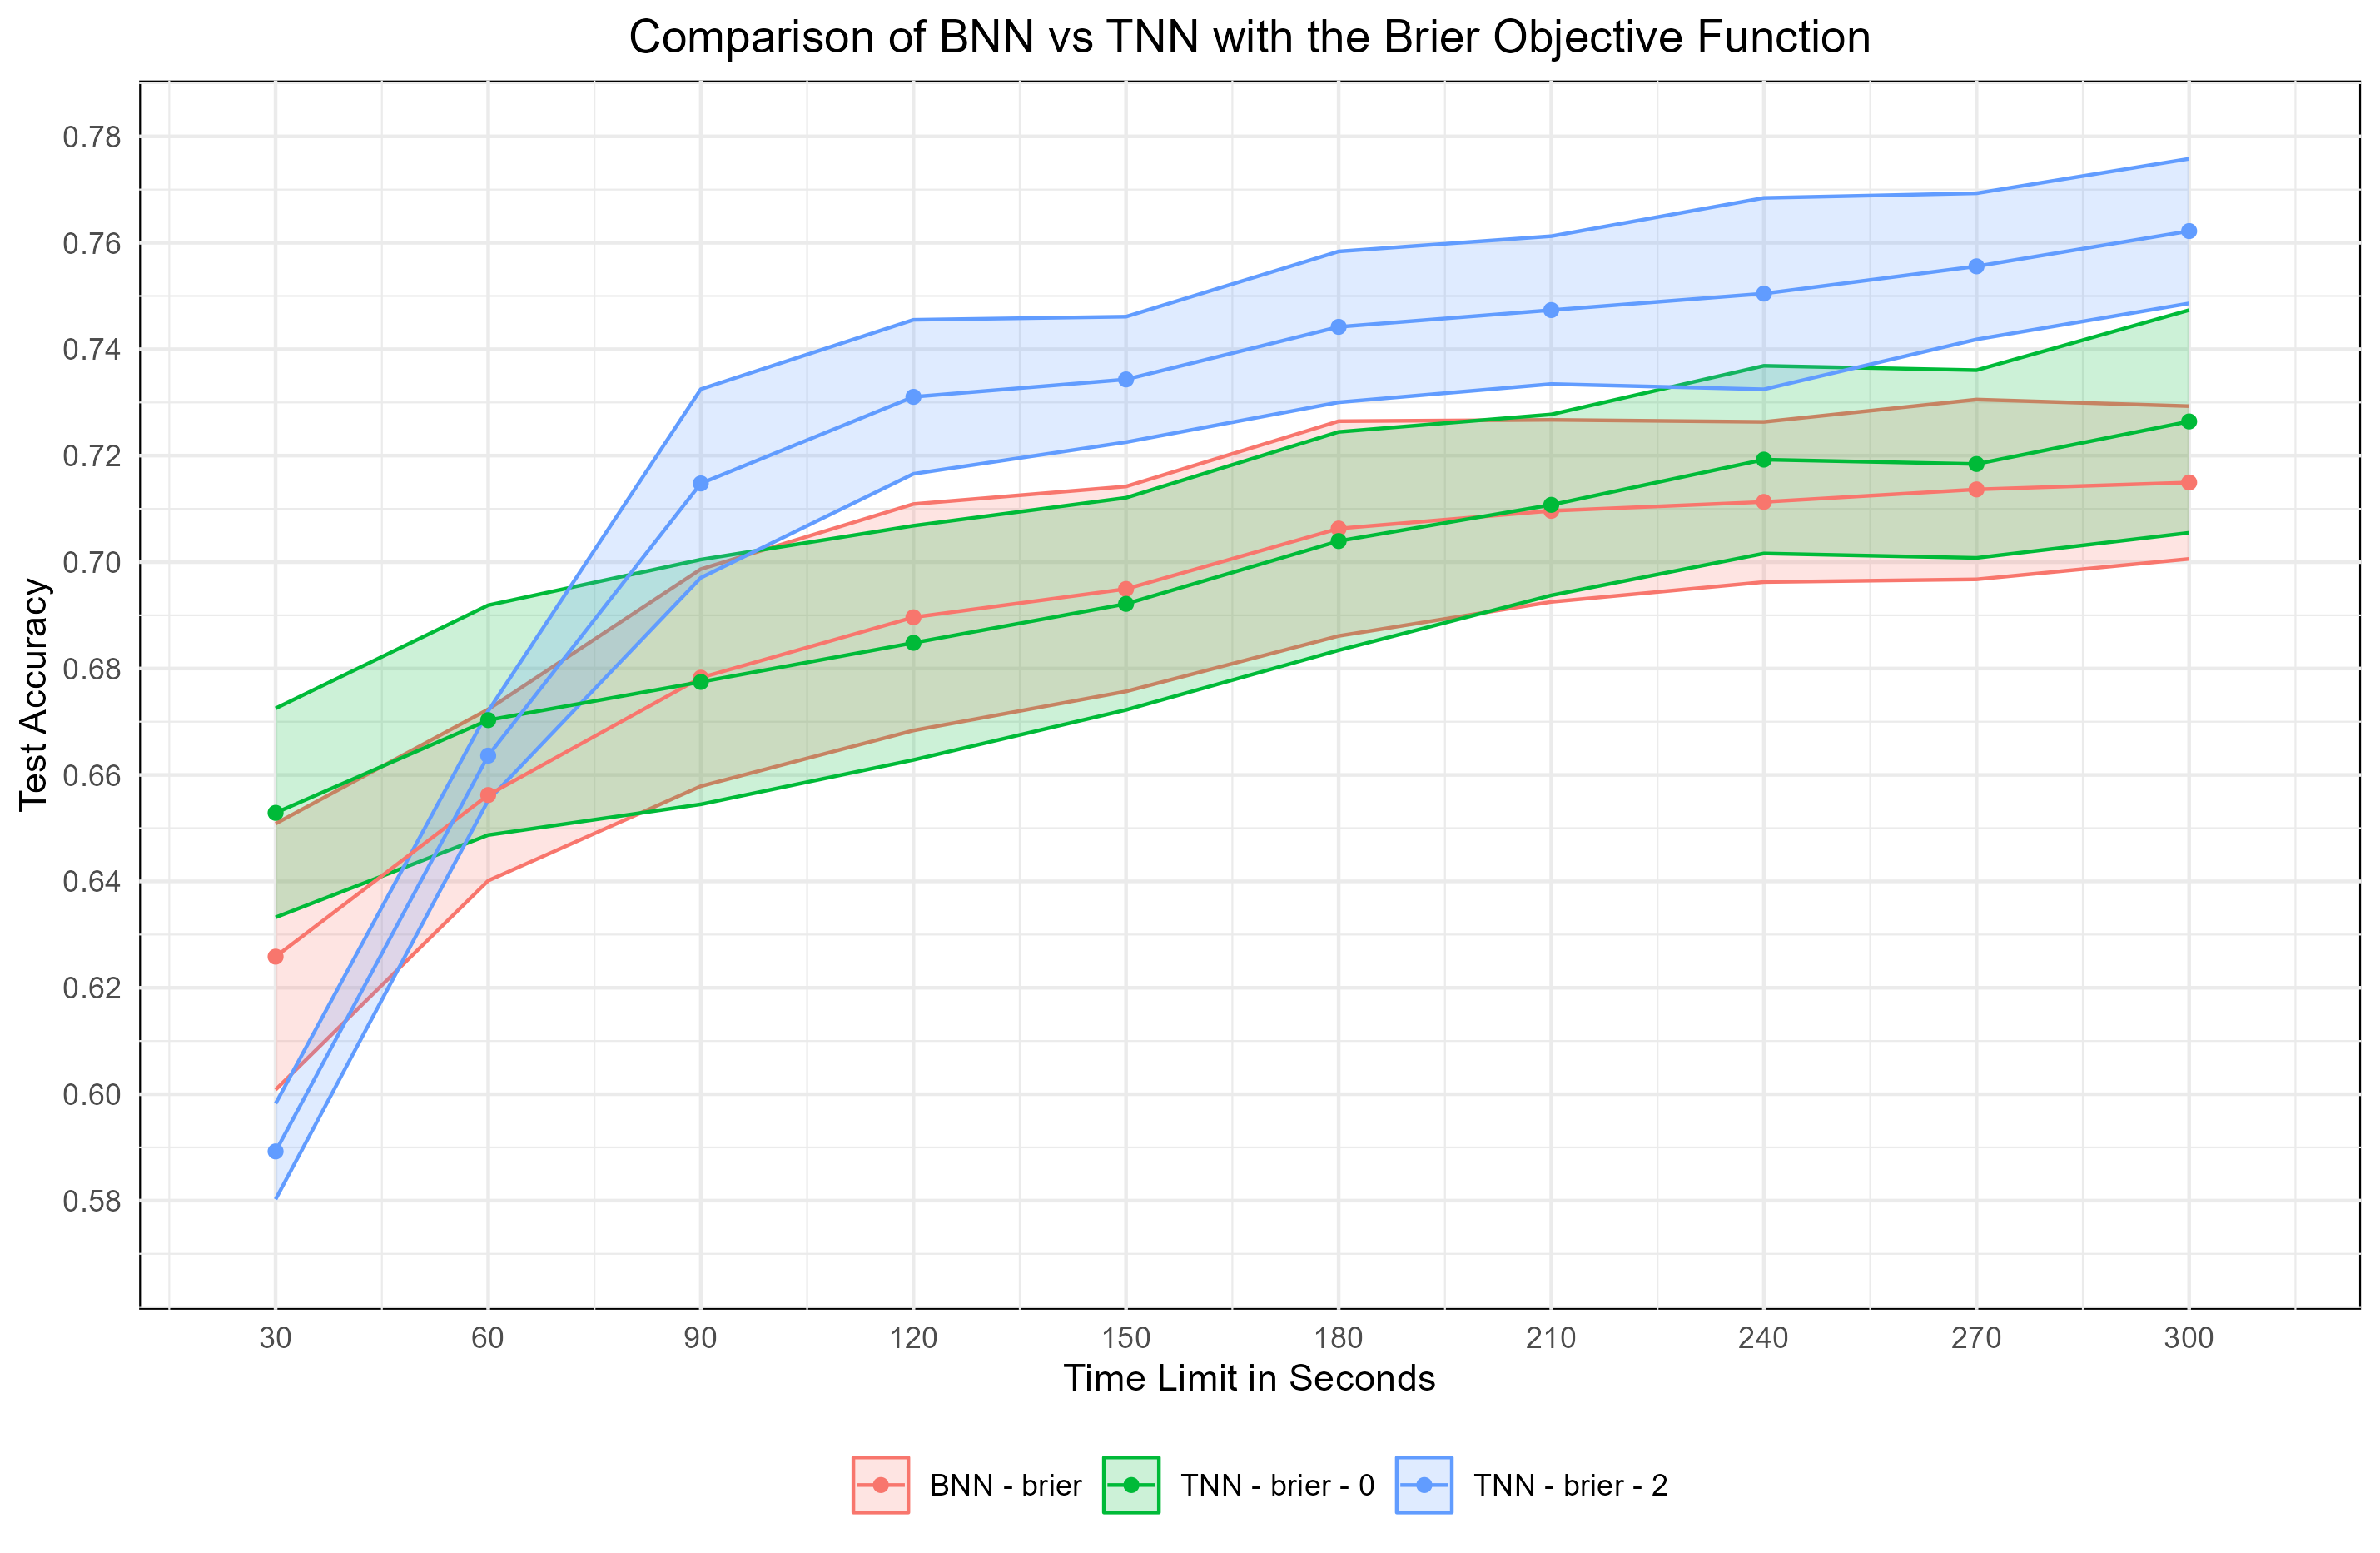
\includegraphics[width=1\linewidth]{Figures/BNN_vs_TNN_brier.png}
    \caption{Test accuracies for the MNIST dataset. The networks are trained on a single batch with 2000 samples, 200 for each digit. The results are for a neural network with a single hidden layer with 16 neurons. The labels indicate what type of network is trained and what the regularization parameter is. The figure shows the mean accuracy of 5 runs as a line and the standard deviation as a shaded area around it.}
    \label{BNN_vs_TNN_brier}
\end{figure}

\begin{figure}[H]
    \centering
    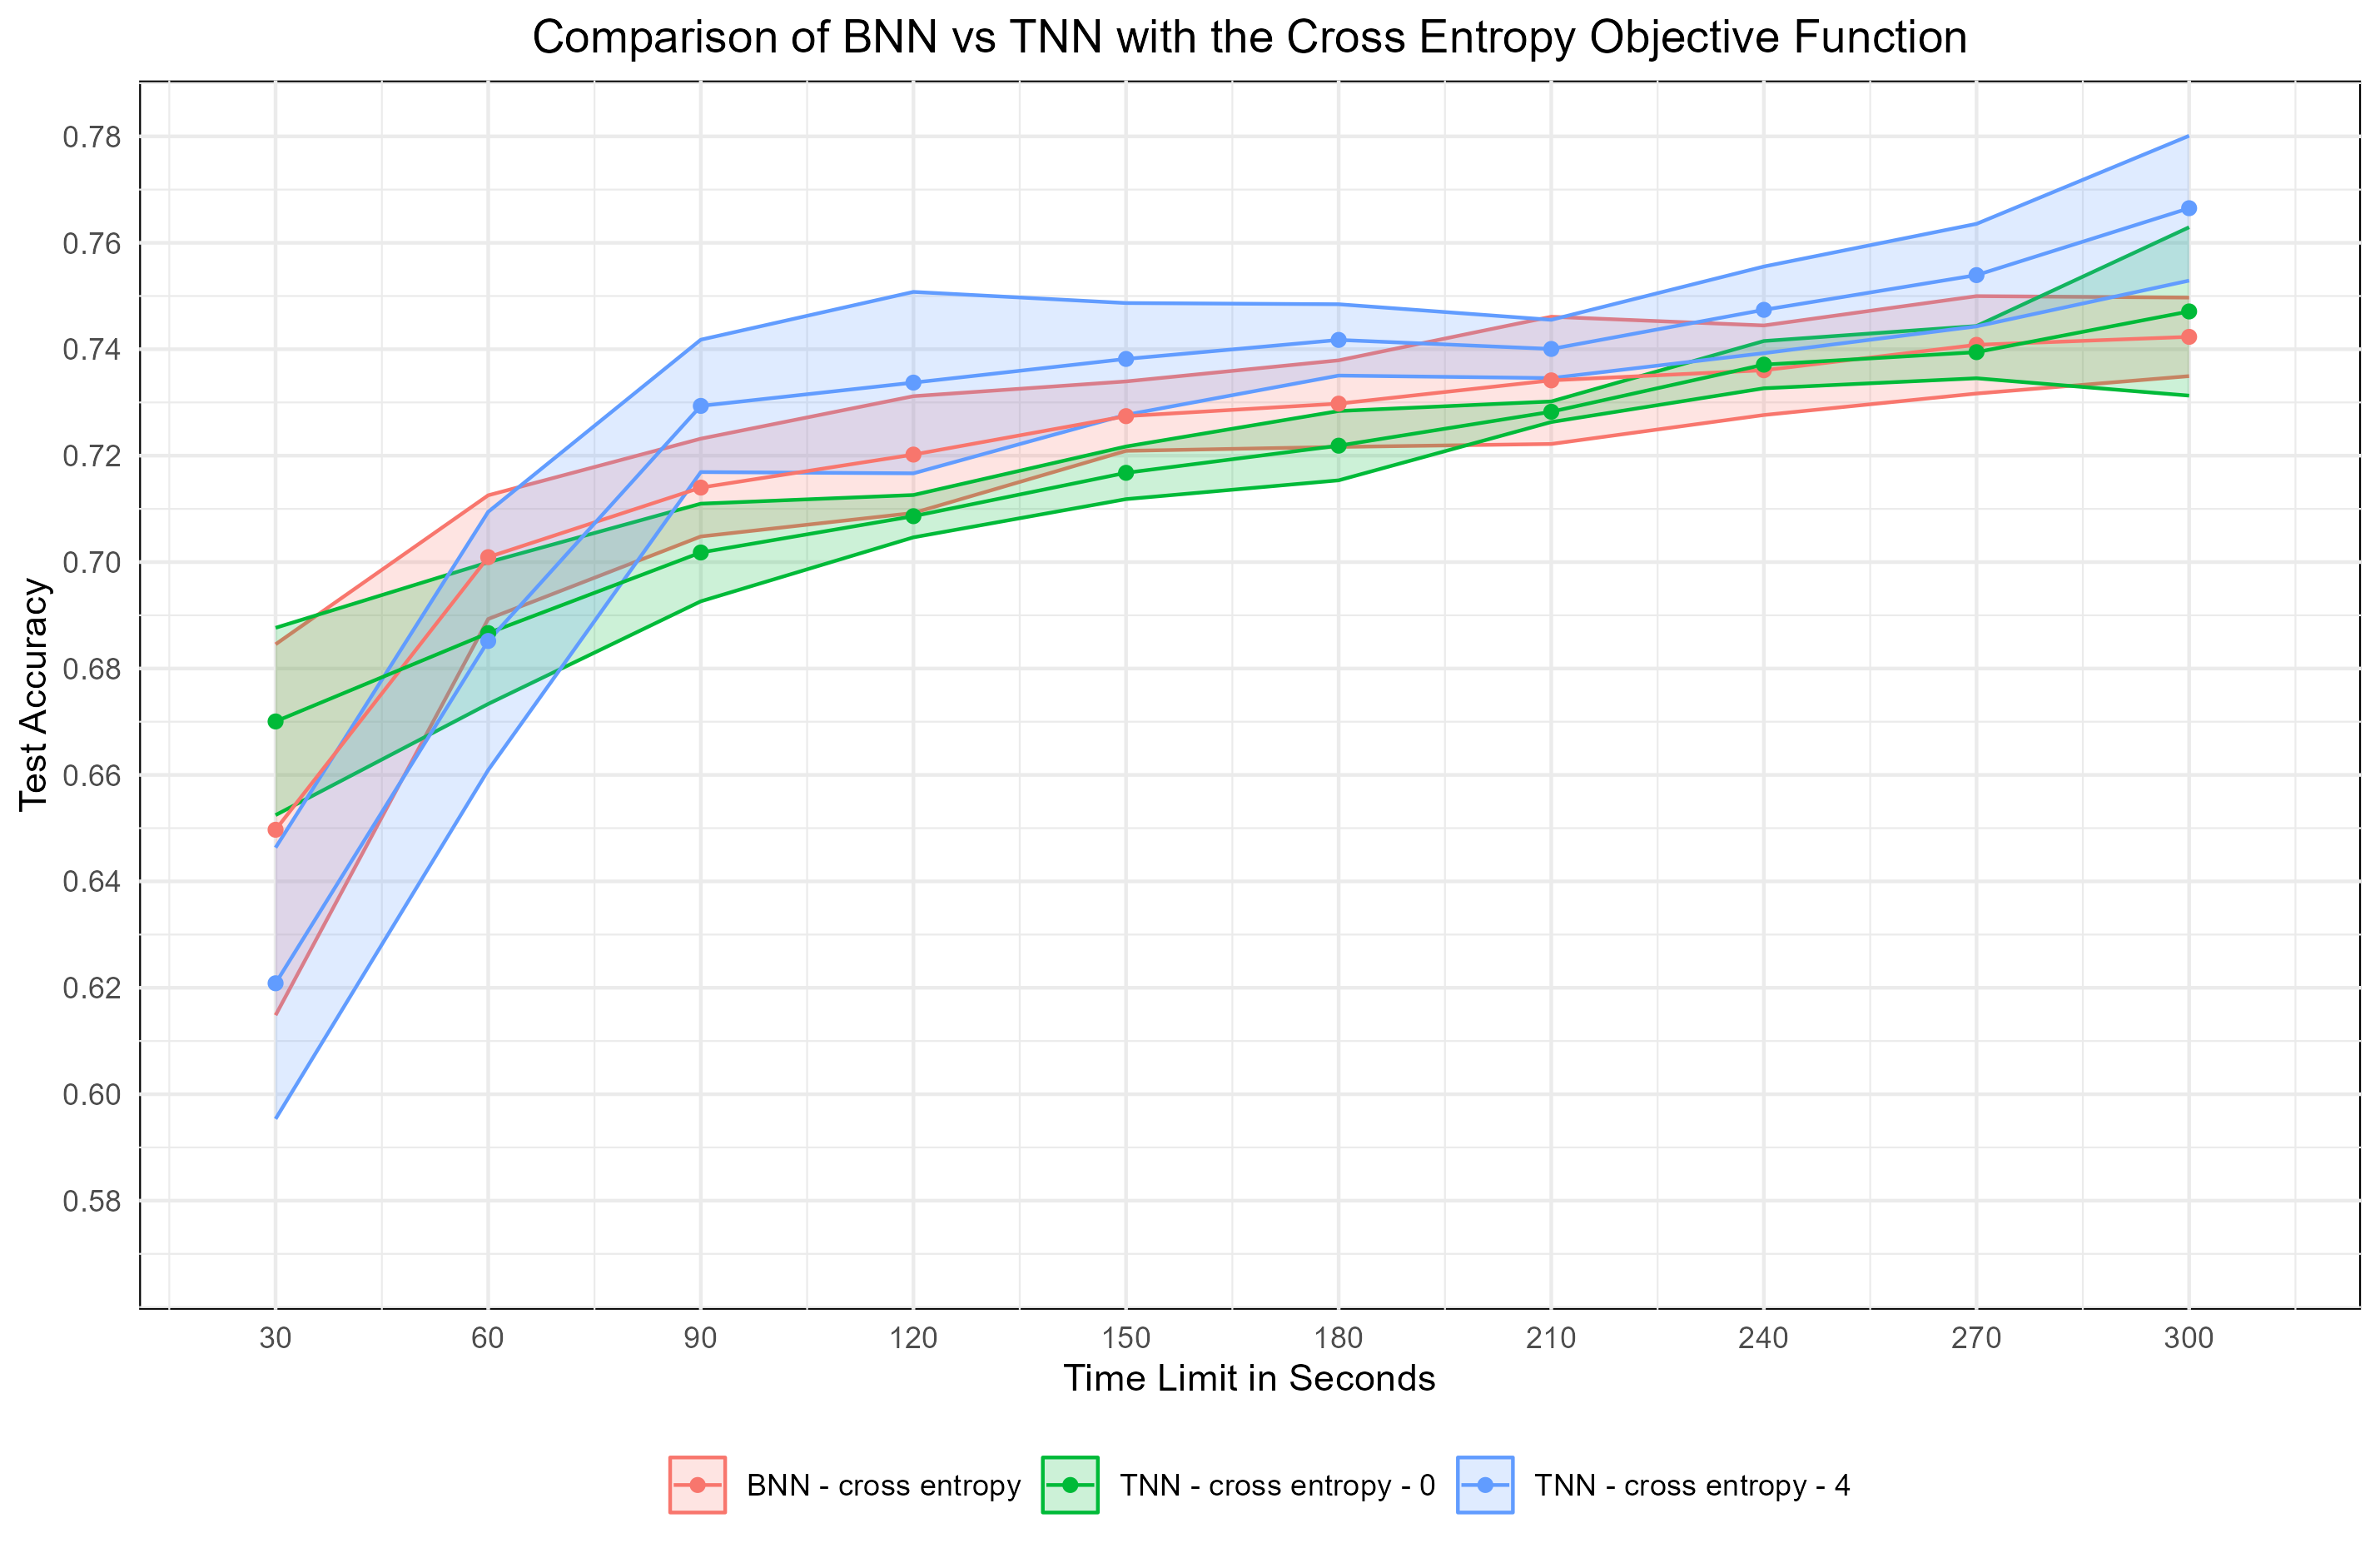
\includegraphics[width=1\linewidth]{Figures/BNN_vs_TNN_cs.png}
    \caption{Test accuracies for the MNIST dataset. The networks are trained on a single batch with 2000 samples, 200 for each digit. The results are for a neural network with a single hidden layer with 16 neurons. The labels indicate what type of network is trained and what the regularization parameter is. The figure shows the mean accuracy of 5 runs as a line and the standard deviation as a shaded area around it.}
    \label{BNN_vs_TNN_cs}
\end{figure}



\subsection{The BeMi Ensemble}
The implementation also support training binary classifiers. As a result it is possible to implement the BeMi ensemble introduced by \cite{ambrogio2023}. In their paper, they test their ensemble for two network architectures, both with two hidden layers. One of them has 4 neurons in both hidden layers, while the other has 10 in the first and 3 in the second. I will try to train networks with the same structure as them, i.e. 10 neurons in the first hidden layer and 3 in the second hidden layer. Besides from this structure, I also train a network with a single hidden layer with 10 neurons. I hypothesize that this architecture is better, as the range of the preactivation values for the neuron in the last layer is larger. Recall, that the BeMi emsemble works by training a binary classifier for each pair of classes. For MNIST, this means that 45 networks must be trained. Again, I use balanced batches to make a fair comparison against the existing literature. \cite{ambrogio2023} report their best average accuracy on MNIST to be 81.66 \%, using 40 images per digit and a total training time of 7.5 hours, as each of the 45 binary classifiers is trained for 600 seconds. \\

\noindent The remaining of this section is structured as follows: At first I start by testing the different objective functions against each other. Afterwards I explore the importance of training data and the effect of the time limit. Lastly, I move on from BNNs to TNNs and see if it is possible to improve on the BNN results. The original BeMi ensemble is trained on TNNs. 

\subsubsection{Comparing Objective Functions} 
For binary classifiers, there is only one neuron at the output layer, so across objective functions the goal is the same, but the values of the objective functions can differ, which might lead to different results. I start by testing the different objective functions. I test with the two network architectures described above. I also test with both 10 and 100 images per digit and with a time limit for each binary classifier of 5 and 10 seconds. The results can be seen in Table \ref{BEMI_OBJ}, where as expected the objective functions give very similar results. For the network with a single hidden layer, the cross entropy gets the highest mean accuracies in 3 out of 4 cases and in the third it is only beaten by 0.02 \% by the Brier objective function, which reaches a mean accuracy of 86.59 \% with 100 images per digit and 10 seconds of training time per classifier, a total training time of 450 seconds. For all configurations the additional training time gives slightly better results, but in general the classifiers are much faster to train than in the work of \cite{ambrogio2023}, despite using more data. 

\begin{center}
% latex table generated in R 4.2.2 by xtable 1.8-4 package
% Fri May 31 11:29:08 2024
\begin{table}[H]
\centering
\begin{tabular}{|c|c|c|c|c|c|c|}
  \hline
ObjFunc & Images & Time & Mean1 & SD1 & Mean2 & SD2 \\ 
  \hline
brier & 100 & 225 & 0.5643 & 0.020748 & 0.3915 & 0.017008 \\ 
   \hline
brier & 100 & 450 & 0.5766 & 0.024475 & 0.3857 & 0.035266 \\ 
   \hline
brier & 1000 & 225 & 0.8569 & 0.004764 & 0.7417 & 0.010035 \\ 
   \hline
brier & 1000 & 450 & 0.8659 & 0.004340 & 0.7470 & 0.013553 \\ 
   \hline
cross-entropy & 100 & 225 & 0.5708 & 0.028872 & 0.3720 & 0.021409 \\ 
   \hline
cross-entropy & 100 & 450 & 0.5851 & 0.029226 & 0.3735 & 0.011863 \\ 
   \hline
cross-entropy & 1000 & 225 & 0.8582 & 0.007717 & 0.7442 & 0.017460 \\ 
   \hline
cross-entropy & 1000 & 450 & 0.8657 & 0.005599 & 0.7483 & 0.012503 \\ 
   \hline
integer & 100 & 225 & 0.5709 & 0.029312 & 0.3733 & 0.025777 \\ 
   \hline
integer & 100 & 450 & 0.5804 & 0.029027 & 0.3844 & 0.015866 \\ 
   \hline
integer & 1000 & 225 & 0.8580 & 0.005094 & 0.7282 & 0.010162 \\ 
   \hline
integer & 1000 & 450 & 0.8633 & 0.004024 & 0.7287 & 0.009162 \\ 
   \hline
\end{tabular}
\caption{Mean accuracies for the BeMi ensemble. Mean1 and SD1 is for a BNN with a single hidden layer with
          10 neurons. Mean2 and SD2 is for a BNN with a hidden layer with 10 neurons followed by a hidden layer
          with 3 neurons. The training time is the total training time, so each of the 45 networks are trained for
          5 and 10 seconds respectively. The number of images, is the total number of images, so there is 10
          and 100 images for each digit respectively. } 
\label{BEMI_OBJ}
\end{table}

\end{center}


\subsubsection{Testing the Effect of More Training Data}
One of the limitations of the MIP model that the BeMi ensemble was originally trained on is the amount of data it can handle. In a LS context, this limitation does not apply in the same way, so it is possible to train on more training data. Figure \ref{BEMI_BS}, shows the importance of more training data, as the test accuracy quickly increases. The figure is with a time limit of only 5 seconds, so it is highly likely that increasing the time limit will yield a even higher accuracy. With 40 images per digit, corresponding to the amount of data \cite{ambrogio2023} use for their best result (81.66 \%), I get a mean accuracy in this experiment of 79.84 \%, despite using way less time than them. It should be noted, that their result was for the network architecture with two hidden layers with only 4 neurons in each, but they do not get a higher accuracy when using the network architecture with 10 neurons in the first hidden layer and 3 in the second. I only use a single hidden layer with 10 neurons, which does not make the network larger compared to their second architecture. A second thing to notice is that I use a BNN in this experiment, so besides the objective function, I do not in any way regularize the model or train it to be more robust. 

\begin{figure}[H]
    \centering
    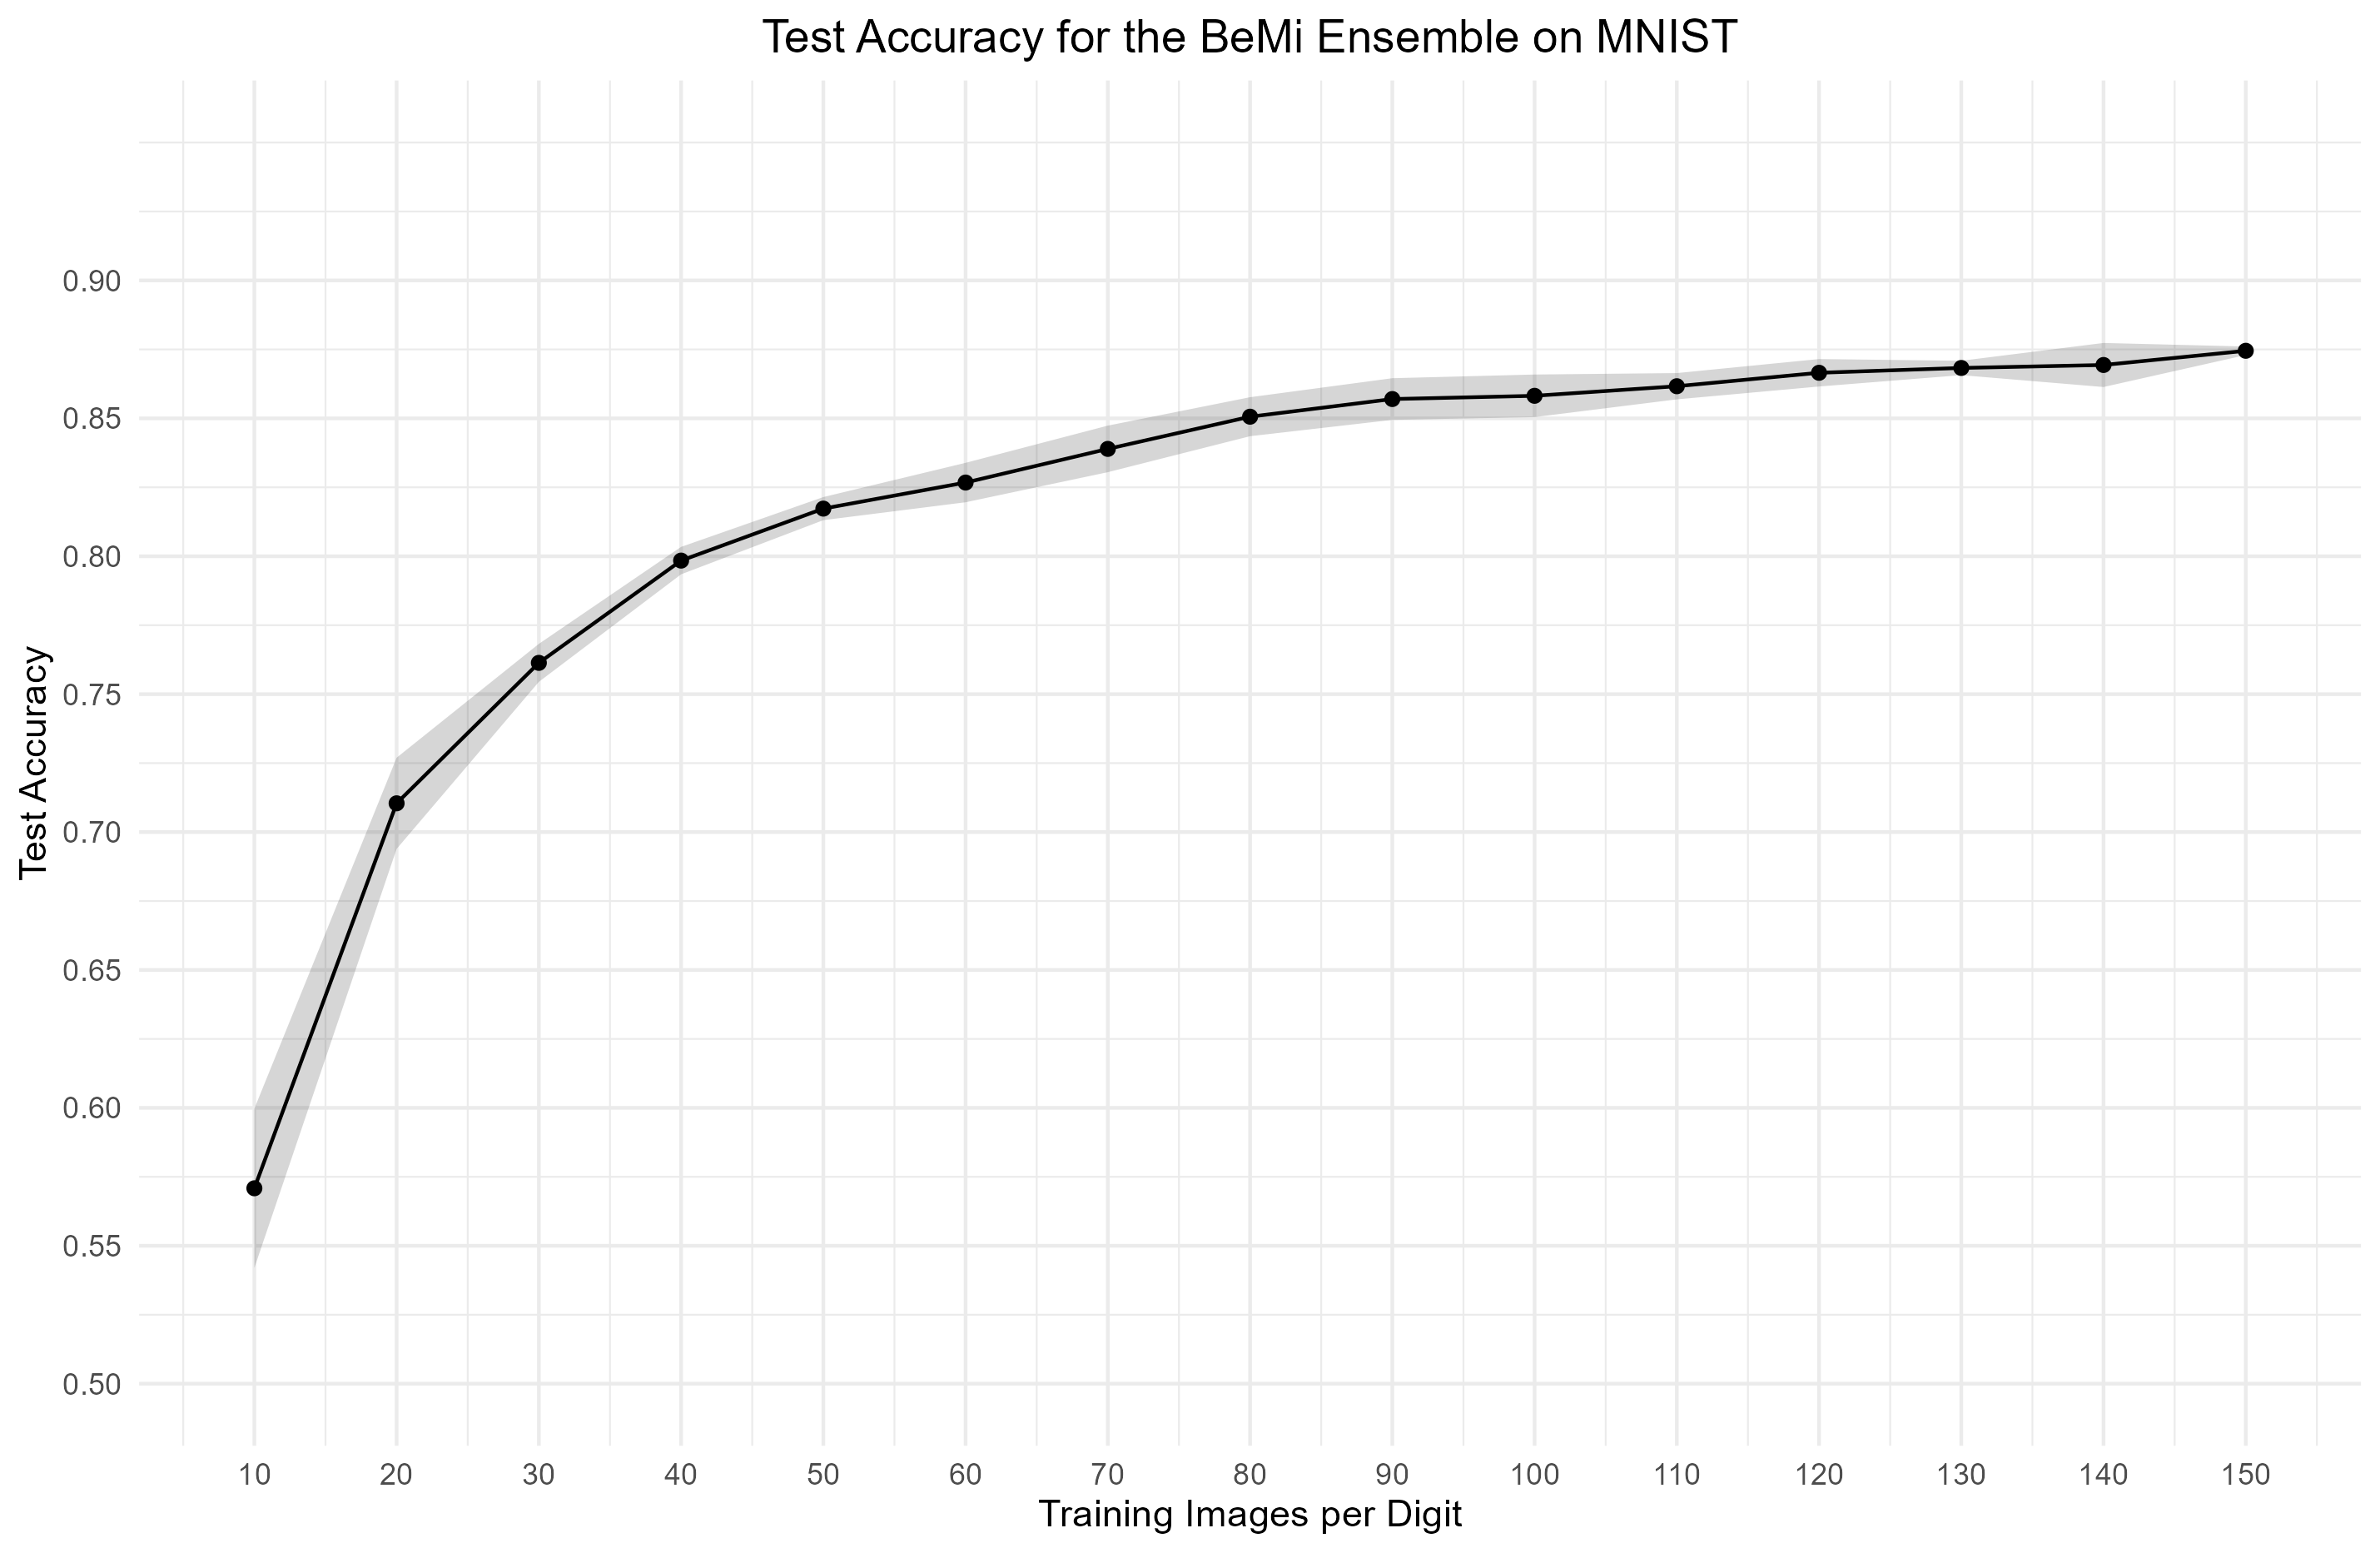
\includegraphics[width=1\linewidth]{Figures/BEMI_BS.png}
    \caption{The test accuracy for the BeMi ensemble as the amount of training data increases. The network is a BNN with a single hidden layer with 10 neurons.
    Each binary classifier is trained for 5 seconds, giving a total training time of 225 seconds. Cross entropy is used as objective function}
    \label{BEMI_BS}
\end{figure}

\subsubsection{Testing the Effect of the Time Limit}
To test how much the results improve as the time limit increases I fix the amount of training data to 100 images per digit and let the time limit vary. Table \ref{BEMI_TIME} shows, that increasing the time limit improve the accuracy slightly and the standard deviation decreases, so the results get more stable. 

\begin{center}
% latex table generated in R 4.2.2 by xtable 1.8-4 package
% Fri May 31 11:47:23 2024
\begin{table}[H]
\centering
\begin{tabular}{|c|c|c|}
  \hline
TrainingTime & Mean & SD \\ 
  \hline
225.00 & 0.8568 & 0.006649 \\ 
   \hline
450.00 & 0.8657 & 0.005599 \\ 
   \hline
675.00 & 0.8669 & 0.005870 \\ 
   \hline
900.00 & 0.8684 & 0.005119 \\ 
   \hline
\end{tabular}
\caption{Summary statistics for the BeMi ensemble for different time limits. The
          network is a BNN with a single hidden layer with 10 neurons and the training is based on
          100 images per digit. I use cross entropy as objective function. } 
\label{BEMI_TIME}
\end{table}

\end{center}


\subsubsection{Using Ternary Neural Networks in the BeMi Ensemble}
As mentioned earlier, in their original publication of the BeMi ensemble, \cite{ambrogio2023} used TNNs for their binary classifiers. So far I have only used BNNs, but in this section I try also with TNNs. I try with different perturbation sizes as well as different weights for the regularization parameter. Table \ref{BEMI_TNN} presents the results for this experiment, and even though the capacity of the model should increase none of the configurations produce better results than the best one achieved in Table \ref{BEMI_TIME}, where the maximum mean accuracy was 86.84 \%. Further, it does not seem to be the case that adding a regularization parameter helps. It might be, that the best weight for the regularization parameter has not been found. The experiments earlier (Table \ref{TNN_COF}, \ref{TNN_REG_BRIER}, \ref{TNN_REG_CS}, and \ref{TNN_REG_INT}), showed how difficult it is to find an optimal regularization parameter. 

\begin{center}
% latex table generated in R 4.2.2 by xtable 1.8-4 package
% Sun Jun  2 22:08:24 2024
\begin{table}[H]
\centering
\begin{tabular}{|c|c|c|c|}
  \hline
Reg & PS & Mean & SD \\ 
  \hline
0.0000 &  10 & 0.8585 & 0.0070 \\ 
   \hline
0.0000 &  30 & 0.8673 & 0.0059 \\ 
   \hline
0.0000 &  50 & 0.8679 & 0.0031 \\ 
   \hline
0.0001 &  10 & 0.8489 & 0.0053 \\ 
   \hline
0.0001 &  30 & 0.8529 & 0.0042 \\ 
   \hline
0.0001 &  50 & 0.8528 & 0.0030 \\ 
   \hline
0.0010 &  10 & 0.8510 & 0.0028 \\ 
   \hline
0.0010 &  30 & 0.8509 & 0.0048 \\ 
   \hline
0.0010 &  50 & 0.8517 & 0.0046 \\ 
   \hline
0.0100 &  10 & 0.8449 & 0.0056 \\ 
   \hline
0.0100 &  30 & 0.8489 & 0.0024 \\ 
   \hline
0.0100 &  50 & 0.8446 & 0.0088 \\ 
   \hline
\end{tabular}
\caption{\small{\textbf{Summary statistics for the BeMi ensemble on MNIST when trained with different perturbation sizes and 
          different regularization parameters. The networks trained has a single hidden layer with 10 neurons and is trained for
          20 seconds each, so the total training time is 900 seconds.}}} 
\label{BEMI_TNN}
\end{table}

\end{center}

\subsection{Testing on Other Datasets}
So far I have only trained on the MNIST dataset. In this section I train on two other datasets as well, namely the more challenging Fashion-MNIST (FMNIST) dataset and the Adult dataset. The structure of the FMNIST dataset is the same as for the MNIST. The training set has 60,000 examples and the test set 10,000 examples. Each example is a $28 \times 28$ grayscale image, but where the MNIST is handwritten digits, the FMNIST is of Zalando articles divided into 10 classes. The task with the Adult dataset is to predict whether the income of an individual exceed 50,000 dollars a year based on census data. This dataset has 14 features, but since some of them are categorical, the number of inputs to the neural network is 104 after standardizing the features. I repeat some of the experiments made so far for these datasets to see if the conclusions drawn so far generalize to these datasets as well. 

\subsubsection{Results on the Fashion-MNIST Dataset}
For the FMNIST dataset, I start by running an experiment on a single batch setting similar to Table \ref{SBT_DNS}. This time I only use one hidden layer, but I still test three objective functions. I train on 2,000 examples. Table \ref{SBT_DNS_FMNIST} present the results for the FMNIST dataset. For the MNIST case, it was the cross entropy objective function that performed best with a small network architecture, whereas for the FMNIST, the Brier objective function performs a little better. For the large network architecture it is, however, again the cross entropy function performing best. 

\begin{center}
% latex table generated in R 4.2.2 by xtable 1.8-4 package
% Sun Jun  2 00:23:15 2024
\begin{table}[!b]
\centering
\begin{tabular}{|c|c|c|c|}
  \hline
ObjectiveFunction & Neurons & Mean & SD \\ 
  \hline
brier & 16 & 0.7016 & 0.0040 \\ 
   \hline
cross-entropy & 16 & 0.6891 & 0.0250 \\ 
   \hline
integer & 16 & 0.6977 & 0.0590 \\ 
   \hline
brier & 128 & 0.6426 & 0.0492 \\ 
   \hline
cross-entropy & 128 & 0.7434 & 0.0060 \\ 
   \hline
integer & 128 & 0.7215 & 0.0115 \\ 
   \hline
\end{tabular}
\caption{\small{\textbf{The mean test accuracies on Fashion-MNIST for different network structures. The results are obtained by training a BNN
            on a single batch with 2000 samples using the ILS algorithm with a time limit of 300 seconds.
            The network is a BNN with a single hidden layer with the number of neurons indicated by the 'Neurons' column.}}} 
\label{SBT_DNS_FMNIST}
\end{table}

\end{center}

